% 设置 biblatex 额外选项
% \PassOptionsToPackage{gbpub=false, gbtype=false}{biblatex}

% 载入 SJTUThesis 模版
% \documentclass[degree=doctor, zihao=-4, language=english, review]{sjtuthesis}
\PassOptionsToPackage{gbpub=false, gbtype=false}{biblatex}
\documentclass[degree=master, zihao=-4]{sjtuthesis}
% \documentclass[degree=bachelor, openany, oneside]{sjtuthesis}
% \documentclass[degree=course, language=english, openright, twoside]{sjtuthesis}
% 选项
%   degree=[doctor|master|bachelor|course],     % 必选,学位类型
%   language=[chinese|english],                 % 可选(默认:chinese),论文的主要语言
%   bibstyle=[gb7714-2015|gb7714-2015ay|ieee],  % 可选(默认:gb7714-2015),参考文献样式
%   review,                                     % 可选(默认:关闭),盲审模式

% 所有其它可能用到的包都统一放到这里了,可以根据自己的实际添加或者删除。
\usepackage{sjtuthesis}
\usepackage{xcolor}
\usepackage{graphicx}
\usepackage{booktabs}
\usepackage{longtable}
\usepackage{minted}
\usepackage{lipsum}
\usepackage[ruled,linesnumbered]{algorithm2e}
%\usepackage{algpseudocode}
\usepackage{hyperref}

% \usepackage{etoolbox}
% \usepackage{xparse}
% \usepackage{environ}
% \usepackage{geometry}	%使用geometry设置页面
% \usepackage{fancyhdr}	%使用fancyhdr设置页眉页脚
% \usepackage{pageslts}	%使用pageslts设置页码格式
% \usepackage{amsmath}	%使用amsmath处理数学公式
% \ifsjtu@setlatinfont@math
% 	\usepackage{unicode-math}
% \fi
% \usepackage{anyfontsize}

% \usepackage{caption}
% \usepackage[backend=biber,style=\sjtu@bibstyle]{biblatex}	%参考文献支持宏包
% \usepackage[titles]{tocloft}	%使用tocloft设置目录格式
% \usepackage[inline]{enumitem}	%更好的列表环境
% \usepackage{pdfpages}	% 便于插入扫描版的原创性声明和授权声明PDF文档
%\includepdfset{fitpaper=true}

%\usepackage{gbt7714}



% 定义图片文件目录与扩展名
\graphicspath{{figure/}}
\DeclareGraphicsExtensions{.pdf,.eps,.png,.jpg,.jpeg}

% 导入参考文献数据库
\addbibresource{bib/ref.bib}

% 信息录入,必须在导言区进行!
% !TEX root = ../thesis.tex

%TC:ignore

\title{有缺失得分和隐性反馈行为特征的动漫推荐系统}
\author{滕启迪}
\studentid{117071910077}
\supervisor{罗珊}
% \assisupervisor{某某教授}
\degree{应用统计专业硕士学位}
\major{应用统计}
\department{数学科学学院}
\date{2020年1月6日}
% \fund{国家 973 项目 (No. 2025CB000000) \\ 国家自然科学基金 (No. 81120250000)}
\keywords{上海交大, 饮水思源, 爱国荣校}

\entitle{Anime Recommender System with Missing Scores and Implicit Feedback Behavior Features}
\enauthor{Qidi Teng}
\ensupervisor{Shan Luo}
% \enassisupervisor{Prof. Uom Uom}
\endegree{Master of Applied Statistics}
\enmajor{Applied Statistics}
\endepartment{School of Mathematical Sciences}
\endate{Jan. 6th, 2020}
% \enfund{National Basic Research Program of China (Grant No. 2025CB000000) \\
%   National Natural Science Foundation of China (Grant No. 81120250000)}
\enkeywords{SJTU, master thesis, XeTeX/LaTeX template}

%TC:endignore


% 自定义项目标签名称
% \sjtuSetLabel{
%   listfigure = {图\quad 录},
%   listtable  = {表\quad 录}
% }

\begin{document}

% 无编号内容:中英文论文封面、授权页
\maketitle
%\makeDeclareOriginality[pdf/originality.pdf]
%\makeDeclareAuthorization		

% 使用罗马数字对前言编号
\frontmatter

% 摘要
% !TEX root = ../thesis.tex

\begin{abstract}
  随着信息过载时代的到来,用户想要从海量信息中找到自己感兴趣的信息变得十分困难,而推荐系统可以通过分析用户历史行为,挖掘用户行为模式,找出用户行为特征并对用户偏好做出预测。真实世界的用户行为数据通常存在很多的问题,诸如数据的稀疏性,隐性反馈行为特征,冷启动问题等等,而解决这些问题也显得尤为重要。本文将基于真实世界的一个用户行为数据集,构建一个为用户推荐动漫的推荐系统,通过多种基本的推荐召回算法实现不同的推荐目的,再利用机器学习技术把多种算法的结果组合起来进行排序以获得更好的效果。同时,采用KNN填充和基于邻域的评分预测有效地解决了稀疏性问题,并通过结合隐式反馈特征和显式反馈特征的方法,选取更合适的样本构造规则。

  \keywords{推荐系统; 协同过滤; 机器学习; 缺失值; 隐反馈特征}
\end{abstract}

\begin{enabstract}
  With the arrival of the era of information overload, it becomes quite difficult for users to find information they are interested in from the huge amount of information. However, the recommender system can find out the user behavior characteristics through analyzing the users' historical behavior and mining user behavior patterns, and then make predictions on users' preferences. There are many problems in real-world user behavior data, such as data sparsity, implicit feedback behavior features, cold start problems, etc, and it is also important to solve these problems. In this thesis, we will build a recommender system based on a real-world user behavior data set, to recommend animation for users. We will choose a variety of basic recommendation recall algorithms to achieve different recommendation goals, and then make use of machine learning technology to sort the combination result of these algorithms for a better behavior. As for the existing problems mentioned above, KNN filtering and neighborhood-based scoring prediciton are used to solve the problem of score data sparsity effectively, and a more appropriate sample construction rule is selected by taking both explicit and implict feedback feature into consideration.

  \enkeywords{Recommender Systems; Collaborative Filtering; Machine Learning; Missing Value; Implicit Feedback Features}
\end{enabstract}


% 目录、插图目录、表格目录
\tableofcontents
\listoffigures
\listoftables
%\listofalgorithms

% 主要符号、缩略词对照表
%% !TEX root = ../thesis.tex

%TC:ignore

\begin{nomenclature}{rl}
\label{chap:symb}
  $\epsilon$     & 介电常数 \\  
  $\mu$ 		& 磁导率 \\
  $\epsilon$     & 介电常数 \\
  $\mu$ 		& 磁导率 \\
  $\epsilon$     & 介电常数 \\
  $\mu$ 		& 磁导率 \\
  $\epsilon$ 	& 介电常数 \\
  $\mu$ 		& 磁导率 \\
  $\epsilon$     & 介电常数 \\
  $\mu$ 		& 磁导率 \\
  $\epsilon$     & 介电常数 \\
  $\mu$ 		& 磁导率 \\
  $\epsilon$     & 介电常数 \\
  $\mu$ 		& 磁导率 \\
  $\epsilon$ 	& 介电常数 \\
  $\mu$ 		& 磁导率 \\
  $\epsilon$     & 介电常数 \\
  $\mu$ 		& 磁导率 \\
  $\epsilon$     & 介电常数 \\
  $\mu$ 		& 磁导率 \\
  $\epsilon$     & 介电常数 \\
  $\mu$ 		& 磁导率 \\
  $\epsilon$ 	& 介电常数 \\
  $\mu$ 		& 磁导率 \\
  $\epsilon$     & 介电常数 \\
  $\mu$ 		& 磁导率 \\
  $\epsilon$     & 介电常数 \\
  $\mu$ 		& 磁导率 \\
  $\epsilon$     & 介电常数 \\
  $\mu$ 		& 磁导率 \\
  $\epsilon$ 	& 介电常数 \\
  $\mu$ 		& 磁导率 \\
  $\epsilon$     & 介电常数 \\
  $\mu$ 		& 磁导率 \\
  $\epsilon$     & 介电常数 \\
  $\mu$ 		& 磁导率 \\
  $\epsilon$     & 介电常数 \\
  $\mu$ 		& 磁导率 \\
  $\epsilon$ 	& 介电常数 \\
  $\mu$ 		& 磁导率 \\
  $\epsilon$     & 介电常数 \\
  $\mu$ 		& 磁导率 \\
  $\epsilon$     & 介电常数 \\
  $\mu$ 		& 磁导率 \\
  $\epsilon$     & 介电常数 \\
  $\mu$ 		& 磁导率 \\
  $\epsilon$ 	& 介电常数 \\
  $\mu$ 		& 磁导率 \\
  $\epsilon$     & 介电常数 \\
  $\mu$ 		& 磁导率 \\
  $\epsilon$     & 介电常数 \\
  $\mu$ 		& 磁导率 \\
  $\epsilon$     & 介电常数 \\
  $\mu$ 		& 磁导率 \\
\end{nomenclature}

%TC:endignore


% 使用阿拉伯数字对正文编号
\mainmatter

% 正文内容
% !TEX root = ../thesis.tex

\chapter{绪论}
  \section{研究背景及意义}
  随着互联网的快速普及和信息技术的高速发展,信息资源正呈现着爆炸式的增长,不论何时何地,人们都可以非常方便地通过互联网来获取信息。2018年天猫“双11”活动,每秒创建订单峰值高达惊人的49.1万笔;今年8月,网易的二季度财报披露网易云音乐的总用户数已经超过了8亿,而这一数字在两年前是4亿,三年前仅是2亿。明显地,人们正在从原先的信息匮乏时代,逐渐地步入信息过载时代。而这个信息过载的时代,不论是对于信息的生产方,还是对于我们这样普通的信息消费方,都带来了巨大的挑战。一方面,对于信息的消费方普通用户而言,面对这海量的数以万计甚至百万计的物品,倘若没有一个明确的需求目标,想要找到对我们有用的,或是我们感兴趣的物品会变得十分困难。而另一方面,对于信息的生产提供方商家而言,如何从这海量的商品库存中,为用户准确地推荐可能符合他们需求的物品,从而自己能够获得收益,这也是十分困难的。在这样的大环境下,推荐系统(Recommender Systems, RS)便应运而生,它主要解决的就是上面所提到的用户-商家双向问题。以电子商务领域为例,推荐系统一方面可以为用户产生个性化的推荐,使得消费者发现对自己有价值的或是感兴趣的物品,进而促进消费者购买欲望,提高其对商家的粘性;另一方面,也有助于商家对用户进行需求分析,从而准确地把握市场需求,带来盈利\cite{卢棪2016协同过滤推荐系统研究及其应用},从而实现用户和商家的互利共赢。

  个性化推荐系统,与我们熟知的搜索引擎类似,都是帮助用户发现信息的一种工具。两者最大的区别在于是否需要用户进行明确输入\cite{2012推荐系统实践}:搜索引擎需要用户输入关键词,然后才能进行搜索,如果想要的东西不能很明确的通过一个或多个关键词进行描述的话,搜索引擎便无法很好工作;而推荐系统不需要用户提供显式的输入,它的核心原理是挖掘用户的行为模式,通过对海量的用户历史行为数据进行分析,然后建立模型,通过模型来预测每个用户的兴趣爱好,最终为不同的用户推荐不同的“个性化”物品。也正是因为这种工作原理,推荐系统通常不会像搜索引擎一样独立的成为一个网站,如百度、Google等等,而是会存在于每个网站的不同应用或是模块的背后,为这些应用和模块的正常工作而服务。

  目前,推荐系统已经在国内外许许多多的领域内有着非常广泛而成功的应用:电子商务网站,如淘宝、京东的商品个性化推荐页面;视频网站,如Youtube首页的推荐视频;社交网络,如新浪微博的热门推荐;音乐电台,如网易云音乐的每日歌曲推荐/私人FM等等。在这些领域内,推荐系统的实际应用也为公司带来了庞大的经济收益。著名的北美在线视频服务提供商Netflix,其自己估计每年通过个性化推荐系统为自身业务节省了约10亿美金\cite{gomez2016netflix};著名电子商务网站Amazon也曾披露,其销售额有20\%-30\%是来自推荐系统。正因如此,对推荐系统的研究在学术界也是越来越受到学者们的关注,并成为了一个比较热门的方向。同时由于其和不同的学科研究领域,比如数据挖掘、机器学习、人工智能等都有着一定的联系,这种交叉学科的性质使得推荐系统正在飞速的向前发展。在当下这个信息爆炸的时代,研究推荐系统是很有意义的,对互联网生态的发展也有着一定的意义。

  \section{国内外研究现状}
  1994年,明尼苏达大学的GroupLens研究组设计了第一个自动化的新闻推荐系统GroupLens\cite{resnick1994grouplens}。这个系统首次提出了协同过滤的思想,并且为后世的推荐问题建立了一个形式化的范式,可以算是最早的推荐系统。1997年,Resnick等人\cite{resnick1997recommender}首次提出推荐系统(Recommender System,RS)一词,自此,推荐系统一词被广泛引用,并且推荐系统开始成为一个重要的研究领域。1998年,著名的个性化商城亚马逊(Amazon)提出了基于物品的协同过滤算法(Item-based Collaborative Filtering),在此之前所普遍使用的协同过滤算法都是基于用户的(User-based CF),而Amazon提出的这个新算法的实际效果非常好。2003年,Amazon在IEEE Internet Computing上公开了这个item-CF算法\cite{linden2003amazon},带来了广泛的关注和使用,包括YouTube、Netflix等著名海外公司。2005年Adomavic{}ius等人的综述论文 将推荐系统分为3个主要类别,即基于内容的推荐、基于协同过滤的推荐和混合推荐的方法,并提出了未来可能的主要研究方向\cite{adomavicius2005toward}。

  到了2006年,一个大事件将推荐系统的研究推向了快速发展的高潮阶段:Netflix宣布了一项竞赛,第一个能将现有推荐算法的准确度提升10\%以上的参赛者将获得100万美元的奖金。这个比赛在学术界和工业界引起了很大的关注,吸引了来自186个国家和地区的超过4万支队伍参赛。而在之后的那几年,许多经典的推荐算法被提出,比如:Koren等人对利用矩阵分解(Matrix Factorization, MF)实现协同过滤的现有技术进行了综述\cite{koren2009matrix},包括基本MF原理,以及包含隐反馈、时序动态等特殊元素的MF等;Steffen Rendle等人在2009年提出了一种“基于贝叶斯后验优化”的个性化排序算法BPR\cite{rendle2009bpr},它是采用pairwise训练的一种纯粹的排序算法。

  近年来随着人工智能的火爆,机器学习和深度学习技术也被广泛运用到了推荐系统的排序场景中。Google在2016年最新发布的模型Wide\&Deep\cite{cheng2016wide}就是综合应用了机器学习和深度学习的产物。它将逻辑回归(LR)与深度神经网络(DNN)结合在一起,既发挥了LR强解释性、高效易规模化的优势,又补充了DNN的强泛化与自动特征组合能力。这个方法应用在Google play的推荐场景中并获得了良好的效果;另一个DeepFM模型\cite{guo2017deepfm}则是将传统的因子分解机FM和DNN结合在一起,用来在CTR预估中挖掘构造有用的高级交叉特征。

  除了基本的推荐算法外,关于推荐系统的一些其他方面,比如冷启动问题、缺失数据的填充、隐反馈信息的利用等等,也涌现出不少优秀的研究成果。比如用隐语义模型(LFM)来解决隐性反馈数据的协同过滤问题\cite{hu2008collaborative};用完整数据的协同过滤来预测缺失的得分信息\cite{ren2012efficient};通过最大化TOPK曲线下面积,将缺失得分统一填充为一个较低的数值\cite{steck2010training};利用一种简单的挖掘关联属性的方法来处理Item-based CF中的完全物品冷启动问题\cite{zhang2019addressing}等等。

  \section{研究问题与内容}
  真实世界的用户行为数据集通常存在着以下几个问题:
  \begin{enumerate}
    \item 数据的稀疏性。由于用户和物品的基数庞大,每个用户只会对一小部分的物品有过行为,如给电影打分,购买物品等等,而对于剩下的大量的其他物品,该用户都没有过行为。这样导致我们生成的用户-物品UI矩阵就是一个稀疏矩阵,这会给某些推荐算法预测用户喜好造成困难,导致推荐效果不理想。

    \item 用户的显性与隐性行为。显性行为指的是可以明确反映用户对物品的喜好程度的行为,最有代表性的的显性行为就是打分,打分高说明用户喜欢这个物品,打分低则说明用户不喜欢这个物品。与之对应的,隐性行为就是那些不能明确反映用户喜好程度的行为。以电子商务网站为例,用户给商品打分属于显性行为,而诸如用户对商品的浏览、点击等行为就属于隐性行为。在真实数据集中,隐性行为要远多于显性行为,有效的利用隐性行为特征可以提高推荐的效果。

    \item 冷启动问题,具体地又分为用户的冷启动,以及物品的冷启动。其中,用户的冷启动指的是如何对新用户进行推荐,因为新用户是没有历史行为数据可供我们的推荐系统进行挖掘分析的;而物品的冷启动主要解决的是如何把一个新的物品推荐给用户,因为这个新的物品在所有的历史行为数据中肯定是没有出现过的。
  \end{enumerate}

  本文选取了网络上公开的一个真实世界中的数据集,这个数据集也有着上面提到的这些问题。基于该数据集的基础上,首先探讨比较了多种召回算法的效果与优缺点;然后将机器学习技术应用于推荐模型的排序阶段,对召回结果进行精排,比较精排后与精排前的效果;然后对于稀疏打分问题,采用KNN填充和基于邻域的评分预测的方法来填补缺失得分;对于隐性反馈行为,采用隐反馈特征和显反馈特征相结合的方法来生成样本标签,基于网格搜索的方法来选择合适的参数组合,并比较处理前后的模型效果。			% 绪论
% !TeX root = ../thesis.tex

\chapter{推荐系统与协同过滤算法简介}
  \section{推荐系统的基本组成}
  在不同业务场景下,推荐系统的设计也会有所差异,但一些必要的组件是共通的。一个普通的推荐系统最主要的组成模块有下面三个:数据层、召回层和排序层。

  \begin{enumerate}
    \item 数据层:推荐系统是在做用户的行为模式挖掘,而挖掘是建立在分析用户对物品的行为数据上的,因此离不开大量数据。数据层其实是一个较为笼统的说法,其主要的功能包括了:上报业务数据、特征工程、数据拼接等等,是推荐算法的数据来源。对于用户行为数据,应尽可能地覆盖用户可能涉及到的业务流程。而对于物品相关的属性数据,也应当尽可能地覆盖更多的属性维度。在推荐系统中,“物品”一词是一种概念性的统称,对于不同的推荐业务场景,“物品”可以指代新闻、小说、音乐、电影等不同对象。用户信息和物品的信息越全,模型最后作出的推荐结果也会越准确。

    \item 召回层:通常推荐模型的计算开销会比较大,而可供推荐的物品数往往成千上万,这样完全依赖模型进行推荐的成本太高。因此设计召回策略是很必要的:将用户可能感兴趣的物品从全量的物品集中事先提取出来,作为推荐内容的候选集,模型最终为每个用户推荐的结果则是这个候选集的某个子集。候选集的大小一般不会很大。
    召回算法种类丰富,如有热门推荐、基于内容/标签等的召回、协同过滤召回、主题模型召回等等。通常来说,单一召回算法得到的结果比较难以满足业务需求,所以实际情况中往往采用多路召回的策略,即每一路召回尽量采取一个不同的策略,召回$K$条物料,$K$值可以根据各算法的实际表现来分配。

    \item 排序层:排序层针对多路召回的结果,利用排序算法进行打分和重排,以更好的反映用户的偏好。通过排序优化用户对召回集的点击行为后,将用户更可能喜欢的物品取出作为最终的推荐列表推荐给用户,提升用户体验。通常会选取模型预测打分最高的前N个物品,这也被称为TopN推荐。排序算法的种类也很丰富,比如有LR,GBDT等机器学习模型,有BPR等排序模型,还有Wide \& Deep, DNN等深度学习模型等。
  \end{enumerate}

  \section{推荐算法的分类}
  Adomavicius等人\cite{adomavicius2005toward}曾对推荐系统的问题有一个范式化的定义:设所有用户集合为$C$,所有可能被推荐的物品集合为$S$,这两个集合都可以非常大。令$u$表示一个效用函数,度量了某物品$s$对某用户$c$的价值:$u:C\times S\rightarrow R$,这里的$R$是一定区间内的非负实数。则对于用户集合$C$中的任意一个用户$c$,我们想要找到物品集合$S$中那个使得效用最大化的物品,即:
  \begin{equation}
  \forall c\in C, s_c^{'}=\mathop{argmax}_{s\in S}u(c,s).
  \end{equation}

  在推荐系统中,这个效用函数通常是一个打分函数,表示用户对物品的喜好程度。
  根据数据源或是推荐策略的不同,推荐系统算法大体上可以分成下面几大类:基于内容的推荐、基于规则的推荐、协同过滤推荐以及混合推荐。其中,协同过滤算法是目前最主流,应用也是最广泛的一类算法。
    \subsection{基于内容的推荐}
    基于内容的推荐算法(Content-based Recommendation)起源于信息检索和信息过滤研究,该方法中,效用函数$u(c,s)$是基于$u(c,s_i)$来估计的,其中$s_i\in S$表示和物品$s$相似的物品。换句话说,这种算法会推荐给用户和他过去历史上交互过、喜欢过的物品相似的物品。具体地,算法会通过对用户历史行为信息的分析,提取出可以表示这个用户的兴趣爱好的特征向量,然后计算用户特征向量与待推荐物品特征向量间的相似度,最后将和用户相似度高的物品推荐给用户\cite{lops2011content}。

    \subsection{基于规则的推荐}
    基于规则的推荐属于大众型的推荐,比如最多用户点击、最多用户收藏等等,类似那些排名榜单的推荐。这种推荐方法不属于“个性化推荐”,但是很适合应对一些冷启动问题,因为基于规则的推荐算法即使缺少某用户或是某物品的历史行为数据,也能够做出推荐结果。

    \subsection{协同过滤的推荐}
    协同过滤的推荐(Collaborative Filtering, CF)是一种利用集体智慧的推荐方法,它通过数据学习用户与物品历史上的交互交集,过滤掉一些不值得推荐的物品如评分较低的物品,或是用户曾有过交互的物品,最后把真正感兴趣的物品推荐给用户。这种方法有许多优点,比如不需要太多专业领域知识、工程易实现等,也是众多推荐算法中应用最广泛的一种算法。根据是否使用机器学习的思想,协同过滤算法可以进一步划分为基于内存的协同过滤(Memory-based CF)和基于模型的协同过滤(Model-based CF)\cite{su2009survey}两大类。
      \subsubsection{基于内存的协同过滤}
      Memory-based CF主要采用启发式的方法进行推荐,关键的步骤在于选取合适的相似度度量函数。根据维度的不同,分为基于用户的{}协同过滤(User-based CF)和基于物品的协同过滤(Item-based CF)。\cite{wang2006unifying}
      \begin{enumerate}
        \item User-based CF的思想是:当某个用户$u$需要个性化推荐的时候,寻找和他兴趣相似的其他一些用户$v_1,v_2,\ldots,v_k$,然后把这些用户喜欢的,但是该用户没有接触过的物品推荐给$u$。对于用户间的相似度计算,User-based CF采用如下简单的余弦相似度:
        \begin{equation}
        sim(u,v)=\frac{|N(u)\cap N(v)|}{\sqrt{|N(u)|\cdot|N(v)|}},
        \end{equation}
        其中记号$N(u)$表示用户$u$喜欢过的物品集合。得到了用户间的相似度矩阵后,就可以对指定用户对指定物品的感兴趣程度进行预测:
        \begin{equation}
        r_{ui} = \sum\limits_{v\in N(i)\cap B(u,k)}sim(u,v)\cdot r_{vi}.
        \end{equation}

        上式中,$B(u,k)$表示和用户$u$相似度最高的$k$个其他用户,$N(i)$是对物品$i$有过行为的用户集合,$r_{vi}$是用户$v$对物品$i$的兴趣程度。(一般是具体的打分)

        \item Item-based CF的思想是:当某个用户$u$需要个性化推荐的时候,寻找该用户历史上曾经喜欢过的物品列表$j_1,j_2,\ldots, j_n$,然后将和这些物品比较相似的其他物品推荐给用户$u$。对于物品间的相似度计算,Item-based CF的做法和User-based CF相仿:
        \begin{equation}
        sim(i,j)=\frac{|N(i)\cap N(j)|}{\sqrt{|N(i)|\cdot|N(j)|}},
        \end{equation}
        其中记号$N(i)$表示喜欢物品$i$的用户集合。得到了物品间的相似度矩阵后,就可以对指定用户对指定物品的感兴趣程度进行预测:
        \begin{equation}
        r_{ui} = \sum\limits_{j\in N(u)\cap B(i,k)}sim(i,j)\cdot r_{uj}.
        \end{equation}

        上式中,$B(i,k)$表示和物品$i$相似度最高的$k$个其他物品,$N(u)$是用户$u$喜欢过的物品集合,$r_{vi}$是用户$v$对物品$i$的兴趣程度。(一般是具体的打分)
      \end{enumerate}

      \subsubsection{基于模型的协同过滤}
      诸如机器学习、数据挖掘算法等“模型”的出现和发展,可以使得推荐系统基于训练数据学会如何识别复杂模式,进而对真实数据的协同过滤任务做出智能的预测。Model-based CF就是应用了一些机器学习的思想,常见的方法有:矩阵分解算法、分类回归算法、图算法、Bayes模型、聚类模型等等\cite{su2009survey}。

      \begin{itemize}
        \item 矩阵分解算法:将数据集变换成一个UI打分矩阵$M_{m\times n}$,共$m$行$n$列,表示$m$个用户对$n$个物品的打分情况。由于稀疏性的问题,这个UI矩阵大部分元素都等于零。这种情况下,如果能估计出矩阵的每个位置元素,就可以实现推荐预测了。以简单但有效的FunkSVD算法\cite{funk2006netflix}为例,我们期望将UI矩阵$M$进行分解:
        \begin{equation}
        M_{m\times n}=P^T_{m\times k}Q_{k\times n}.
        \end{equation}

        对于每一个元素$m_{ij}$,通过矩阵分解后的对应表示应该是:
        \begin{equation}
        m_{ij} = e_i^TP^TQe_j = p_i^Tq_j,
        \end{equation}
      
        用均方差作为损失函数,对于全部的用户和物品组合,我们期望最小化的目标函数就是:
        \begin{equation}
        \mathop{argmin}_{p_i,q_j}\sum_{i,j}\big(m_{ij}-p_i^Tq_j\big)^2.
        \end{equation}

        通过最优化上式,得到分解的矩阵$P,Q$,进而用于推荐预测。

        \item 分类回归算法:把推荐问题转化成传统的机器学习分类/回归问题解决,前者输出概率值并根据概率大小排序推荐;后者预测用户对物品的打分,根据打分高低排序推荐。
      \end{itemize}

      \subsubsection{协同过滤方法的优缺点}
      文献\cite{su2009survey}已经对两大类协同过滤方法各自的优点与缺点有了总结。对于Memory-based CF,其主要优点有易实现性、无需考虑推荐物品的具体内容、容易添加新数据;缺点主要是对稀疏数据敏感、难以应对冷启动问题等。而对于Model-based CF,其主要优点是对稀疏数据不敏感、改善了模型效果;缺点是建立模型的开销较大、在预测表现和可扩展性之间有一个权衡、一些降维算法会损失信息。

    \subsection{混合推荐}
    混合推荐(Hybrid RS),是将协同过滤的推荐和基于内容的推荐结合在一起,这种方法可以帮助避免使用单一类推荐算法所遇到的限制或局限性。例如,基于内容的推荐算法偏好给用户推荐与其历史上喜好类似的物品,这样会导致推荐结果缺乏一定的新颖性;协同过滤推荐在遇到冷启动问题,以及数据稀疏、维度灾难等问题时会比较麻烦等。而如果把这几种算法组合到一种推荐算法中去,就可以取长补短,充分利用各自的优势。常见的混合推荐实现类型有\cite{burke2002hybrid}:
    \begin{itemize}
      \item Weighted:给予每种算法一个权重,最后混合来推荐单独的一个物品
      \item Switching:根据不同场景,系统自动在不同的推荐算法之间选择
      \item Mixed:把不同推荐算法得到的推荐结果,放在一起一同展示给用户
      \item Feature combination:将不同推荐算法产生的数据特征组合在一起作为新的特征
    \end{itemize}

  \section{推荐系统的评价指标}
  这里主要讨论实际应用中常见的TopN推荐(后文实验中也是TopN推荐)。记系统对用户$u$推荐的$N$个物品组成的列表为$R(u)$,用户$u$在测试集上实际喜欢的物品组成的集合为$T(u)$,测试集全体用户集合为$\tilde{U}$。下面列出了在后文中用到的一些评价指标\cite{2012推荐系统实践}:
  \begin{itemize}
    \item 精确率:
    \begin{equation}
    Precision = \frac{\sum\limits_{u\in\tilde{U}}|T(u)\cap R(u)|}{\sum\limits_{u\in\tilde{U}}|R(u)|},
    \end{equation}
    
    \item 召回率:
    \begin{equation}
    Recall = \frac{\sum\limits_{u\in\tilde{U}}|T(u)\cap R(u)|}{\sum\limits_{u\in\tilde{U}}|T(u)|},
    \end{equation}

    \item 准确率(命中率):
    \begin{equation}
    Hit\;rate=\frac{\sum\limits_{u\in\tilde{U}}1_{\{T(u)\cap R(u) \neq\emptyset\}}}{|\tilde{U}|},
    \end{equation}

    \item 覆盖率:
    \begin{equation}
    Coverage = \frac{\big|\cup_{u\in\tilde{U}}R(u)\big|}{|I|}.
    \end{equation}
    
  \end{itemize}

  类比机器学习中二分类问题的评价指标,在TopN推荐中,也有对应的精确率(Precision)和召回率(Recall)。精确率体现了结果推荐列表中有多少比例的物品的确被用户产生了行为;而召回率体现了被用户实际产生行为的物品中有多少比例被包含在了最终的推荐结果中。除精确率和召回率以外,命中率类似$Accuracy$,这里作为一个辅助指标;覆盖率可以反映算法挖掘长尾的能力,所谓长尾效应指的就是小部分的物品占据了大部分的流量,而剩余大部分的物品所处的区域就被称为长尾区域。长尾效应中的主体部分体现的是共性数据,这部分数据很容易被挖掘利用;而长尾部分则是个性化数据的体现\cite{曾洋2017基于电商的长尾推荐的研究与实现}。如果推荐算法的覆盖率越高,说明算法越能够将长尾中的物品推荐给用户,而不仅仅是集中推荐热门的共性物品。
			% 推荐系统与协同过滤算法简介
% !TEX root = ../thesis.tex

\chapter{数据准备与实验设计}
  \section{数据集的简介与清理}
  本文选用Kaggle上公开的一个真实世界数据集,是作者从网站\url{MyAnimeList.net}中爬取到的用户将动漫添加到自己的list中、观看动漫、给动漫评分等一系列行为的数据。下载下来的数据集分成三个部分:用户信息、动漫信息、及用户给动漫打分的信息,作者已经对数据做了一定清洗处理,清洗后的数据集约包含10.87万用户对6600部动漫的3000万条打分记录。用户信息和动漫信息表主要是关于用户和动漫这两个维度的一些固有属性;对于打分行为表,一些比较特殊重要的特征如下:
  \begin{itemize}
    \item my\_watched\_episodes:已观看该动漫集数;
    \item my\_score:打分,取值为0到10之间的整数;
    \item my\_status:观看状态,主要取值有:$\{1:\text{watching},\;2:\text{completed},\;3:\text{on hold},\;4:\text{dropped},\;6:\text{plan to watch}\}$;
    \item my\_last\_updated:最后一次更新状态的日期。
  \end{itemize}

  在作者清洗的基础上,额外进行的清洗工作如下:
  \begin{enumerate}
    \item 删除last\_update\_date字段取值为"1970-01-01"的异常样本;
    \item 删除my\_status字段取值不属于$\{1,2,3,4,6\}$的样本(其他取值具体含义不明,且样本量很少);
    \item 删除last\_update\_date字段取值早于该动漫的最早上映日期的样本;
    \item 结合用户观看集数与该动漫总集数,修正my\_status取值。具体地,若观看集数等于总集数且非零,则令my\_status = 2;若观看集数不等于零,且原本的my\_status = 6(即准备观看),则修改my\_status = 1(观看中);
    \item 最后,由于原始数据集的样本量太大(3000万行,11万用户),单机情况下程序执行有很大困难,因此决定对原始数据集进行抽样。抽样的方法是对11万用户随机抽样5\%,约5500名用户,抽样后的打分行为数据集大小约为151万行。抽样的合理性在后续章节会进行实验分析。
  \end{enumerate}

  \section{训练集和测试集划分}
  本实验目的是利用这些用户行为数据,构建一个为用户推荐他可能感兴趣动漫的推荐系统,这种推荐属于TopN推荐而非评分推荐。具体地,这种推荐的目的是预测用户是否会看某部动漫,而不是预测用户对该动漫打多少分。

  打分行为数据集中的字段last\_update\_date,其含义是用户更新状态的最后一次时间。表~\ref{tab:date_distribution}是对原始数据集和抽样数据集中该字段的分位数分布统计:
  % Table generated by Excel2LaTeX from sheet 'Sheet1'
  \begin{table}[htbp]
    \centering
    \caption{原始和抽样数据集中的日期分布}
    %\textbf{表3.1}~~原始和抽样数据集中的日期分布
      \begin{tabular}{lrr}
      \toprule
      quantile & raw dataset & sampling dataset \\
      \midrule
      10\% & 2009-08-02 & 2009-08-12 \\
      20\% & 2010-12-18 & 2010-12-26 \\
      30\% & 2012-04-17 & 2012-04-16 \\
      40\% & 2013-05-11 & 2013-04-23 \\
      50\% & 2014-04-10 & 2014-03-31 \\
      60\% & 2015-03-08 & 2015-02-26 \\
      70\% & 2015-12-28 & 2015-12-20 \\
      80\% & 2016-09-28 & 2016-09-23 \\
      90\% & 2017-07-24 & 2017-07-16 \\
      \bottomrule
      \end{tabular}%
    \label{tab:date_distribution}%
  \end{table}%

  根据我们要推荐的“物品”,即动漫其本身的季节性特点,通常分为一年四个季度上映,上映日期分别在1月,4月,7月和10月。因此考虑取时间划分节点为"2017-06-30",即last\_update\_date取值小于"2017-06-30"的样本为训练集,剩下的样本为测试集。这样划分下来的训练集/测试集比例大约为9:1。

  \section{正负样本构造}
  划分完训练测试集后,还需要设置样本标签。一方面,各召回算法所利用的“用户历史上喜欢过的动漫”数据,其中的“喜欢”和“不喜欢”即是由样本标签表示;另一方面,应用机器学习技术对召回结果进行重排序是一个有监督模型,因此也需要样本标签。对于TopN推荐,比较合适的重排序是选择一个二分类模型,最后根据模型输出的概率值排序。

  测试集标签设置比较容易。TopN推荐关心的是用户是否观看了系统所推荐的结果,所以对于任意测试样本,只要my\_watched\_episodes不等于零(表示用户看过了这一部动漫),则令样本标签$y=1$,否则$y=0$。

  训练集标签设置相对复杂。从模型训练角度看,正样本应表明用户喜欢看这部动漫,而不仅是“看过”,因此标签的设置依赖于用户对动漫的打分my\_score,打分越高,用户的喜欢程度越大。因为是二分类问题,样本标签$y\in\{0,1\}$。具体的方法是对分数取一个阈值,令打分高于阈值的样本$y=1$,否则$y=0$。表~\ref{tab:status_score_distribution}是数据集中各个status对应的打分分布情况,以及各个分值在网站中的含义:

  \begin{table}[htbp]
    \centering
    \caption{各status对应打分分布情况}
    %\textbf{表3.2}~~各status对应打分分布情况
    \resizebox{\textwidth}{!}{
      \begin{tabular}{lrrrrrr}
      \toprule
      my\_score & \multicolumn{1}{l}{meaning} & 1    & 2    & 3    & 4    & 6 \\
      \midrule
      \multicolumn{1}{r}{1} & \multicolumn{1}{l}{Appaling} & 0.30\% & 0.40\% & 0.30\% & 4.50\% & 8.80\% \\
      \multicolumn{1}{r}{2} & \multicolumn{1}{l}{Horrible} & 0.20\% & 0.50\% & 0.20\% & 4.90\% & 0.10\% \\
      \multicolumn{1}{r}{3} & \multicolumn{1}{l}{Vey bad} & 0.30\% & 0.80\% & 0.50\% & 7.50\% & 0.30\% \\
      \multicolumn{1}{r}{4} & \multicolumn{1}{l}{Bad} & 0.60\% & 1.90\% & 1.40\% & 15.70\% & 0.60\% \\
      \multicolumn{1}{r}{5} & \multicolumn{1}{l}{Average} & 2.90\% & 4.70\% & 6.10\% & 24.20\% & 4.90\% \\
      \multicolumn{1}{r}{6} & \multicolumn{1}{l}{Fine} & 8.30\% & 10.60\% & 16.40\% & 20.00\% & 5.70\% \\
      \multicolumn{1}{r}{7} & \multicolumn{1}{l}{Good} & 21.80\% & 22.30\% & 30.60\% & 14.20\% & 11.80\% \\
      \multicolumn{1}{r}{8} & \multicolumn{1}{l}{Very good} & 27.20\% & 26.50\% & 25.20\% & 5.80\% & 19.20\% \\
      \multicolumn{1}{r}{9} & \multicolumn{1}{l}{Great} & 21.00\% & 19.00\% & 12.10\% & 1.90\% & 13.90\% \\
      \multicolumn{1}{r}{10} & \multicolumn{1}{l}{Masterpiece} & 17.60\% & 13.40\% & 7.20\% & 1.20\% & 34.80\% \\
      proportion &      & 2.37\% & 89.07\% & 2.24\% & 5.92\% & 0.40\% \\
      zero propotion &      & 64.80\% & 12.40\% & 64.60\% & 48.70\% & 98.60\% \\
      \bottomrule
      \end{tabular}}%
    \label{tab:status_score_distribution}%
  \end{table}%

  从表~\ref{tab:status_score_distribution}中可以得出:
  \begin{itemize}
    \item 数据集打分缺失比例较高,特别是my\_status=6的样本几乎全是0分;
    \item 各status平均打分大约在7-8分左右,除去my\_status=4比较低。
  \end{itemize}

  结合上面的结论,训练样本标签设置方法如下:
  \begin{enumerate}
    \item 阈值初设为8分,高于8分为正样本,低于8分且打分非零的为负样本(8分的理由是略高于各状态平均打分);
    \item my\_status=4的零分样本也是负样本(状态4对应放弃观看);
    \item my\_status=1,2,3的零分样本剔除出训练集(后续填充缺失时使用);
    \item my\_status=6的零分样本剔除出训练集(状态6几乎都是0分)。
  \end{enumerate}

  处理之后训练集最终大小约为90万行,正负样本比约为$1.25:1$。

  \section{用户与物品画像表设计}
  原始的用户信息和动漫信息数据集含有许多的类别特征、文本特征。为了能够在后面的机器学习模型中应用这些数据,需要做一定的预处理。对于用户画像特征,主要做的处理有:
  \begin{itemize}
    \item 根据birth\_date,计算用户的年龄age(用"2017-06-30"减去birth\_date,结果向下取整);
    \item 统计每个用户在训练集中各status对应的观测数;
    \item 统计每个用户在训练集中“喜欢”的动漫数(即$y=1$的记录数);
    \item 统计每个用户喜欢的动漫中,各source(原作类型)、各rating(适宜人群)及各genre(流派风格)的占比;
    \item 对之前剔除出的my\_status=6的样本,同样统计每个用户对应上述各特征占比。
  \end{itemize}

  对于物品画像特征,主要做的处理有:
  \begin{itemize}
    \item 将打分人数scored\_by和成员数members合并成一个新字段scored\_ratio;
    \item members的数值区间太大,将其分箱成6个区间,对应不同的流行度;
    \item 适当扩充type字段,把type=TV扩充成长篇、半年番、季番、短篇以及泡面番;
    \item source字段适当精简合并成9类;
    \item genre字段挑选出有代表性的20个流派风格。由于同一部动漫可以同时包含多个genre,还需要对genre做One Hot处理。
  \end{itemize}

  \section{实验设计}
  本文后续实验分为下面几个步骤:
  \begin{enumerate}
    \item 基于随机抽样后的打分行为数据集,采用四种不同召回算法,并比较分析这四种算法的效果差异。然后利用Xgboost
    模型对召回结果进行打分重排,输出最终结果。比较排序后的模型效果和排序前的模型效果差异。
    \item 对随机抽样的可行性分析,设计实验比较抽样、全量与增量训练彼此之间的效果差异。
    \item 对数据稀疏问题,采用KNN填补和基于邻域的评分预测方法,比较填补缺失后的召回算法效果与填补前的差异。
    \item 对隐反馈特征的利用,包括my\_watched\_episodes, my\_status等,将其和my\_score综合考虑来确定样本的标签,并比较模型的效果差异。
  \end{enumerate}	% 实验数据与设计
% !TEX root = ../thesis.tex

\chapter{实验分析}
  \section{基本实验结果}
  基本实验基于对全量用户随机采样5\%后得到的训练集和测试集。根据时间进行划分会出现“新用户”及“新动漫”(下面用“新番”称谓)两个概念。新用户指的是在2017年6月30日之前没有过行为,或是打分均为零的用户;新番指的是首映日期在2017年6月30日之后的动漫。
    \subsection{四种召回算法}
    本实验采用的四种基本召回算法,分别是Item-based CF召回,Item-related召回, 人口统计召回以及Item-similarity召回。其中,Item-based CF召回属于协同过滤算法,人口统计召回属于基于规则的推荐,Item-similarity召回类似基于内容的推荐,而Item-related召回是根据数据集自带特征的特点进行的关联推荐。下面简要介绍一下这四种算法:
      \subsubsection{Item-based CF}
      这个就是前文提过的经典的基于物品的协同过滤算法\cite{wang2006unifying}。算法伪代码见4-1。
      \begin{algorithm}[htbp]
        \caption{Item-based CF}
        \KwIn{$u\in\tilde{U},\;W,\;I(u),\;S(u),\;K_1,\;K_2$}
        \KwOut{$R(u)$}
        $res=\{\},\;R(u)=[]$\;
        \If{$I(u)=\emptyset\;\;\textbf{or}\;\;S(u)=\emptyset$}{
          return $R(u)$\;}
        \For{$i \in I(u)$}{
          $cnt=0$\;
          \For{$j,w_j \in\;sort(W[i])$}{
            \If{$j \in S(u)$}{\textbf{continue}\;}
            $res[j]\leftarrow res[j]+w_j$\;
            $cnt\leftarrow cnt+1$\;
            \If{$cnt\geq K_1$}{\textbf{Break}\;}
          }
        }
        $R(u)=sort(res,K_2)$\;
        return $R(u)$\;
      \end{algorithm}
      符号说明:$\tilde{U}$是全体测试集用户;$W$是物品相似度矩阵;$I(u)$是用户$u$在训练集中喜欢的动漫集合;$S(u)$是用户$u$在训练集中观看过的动漫集合;$K_1,K_2$分别是选取的邻域大小以及最终召回的动漫个数;$R(u)$是最后为用户$u$召回的动漫集合。

      \subsubsection{Item-related召回}
      动漫信息数据集中的字段related存储了与该动漫相关联的其他动漫、漫画及关联方式。涉及的关联方式主要有:
      \begin{itemize}
        \item Adaptation:改编,占所有related key比例的30\%。但是通过
        Adaptation关联得到的都是漫画,而漫画不包含在我们的推荐目标范围内(数据集局限于TV动画、OVA、Movie等);
        \item Sequel/Prequel:续集/前传,二者一一对应,占所有related key比例的28\%。通常动漫A的OVA会作为A的Sequel关联;
        \item Parent story/Side story:父篇/番外,二者也是一一对应,占所有related key比例的15\%。
      \end{itemize}
      Item-related召回就是根据Sequel、Prequel、Parent story和Side story这四种related key来进行关联推荐。具体的召回的方法是:对每个用户历史上喜欢的动漫按照打分从高到低排序,然后依次通过related方式关联到新的动漫(可能没有关联),如果关联到的这部动漫没有被用户看过,就加入召回列表。算法伪代码见4-2:
      \begin{algorithm}[htbp]
        \caption{Item-related Recall}
        \KwIn{$u\in\tilde{U},\;Re,\;I(u),\;S(u),\;K$}
        \KwOut{$R(u)$}
        $R(u)=\{\}$\;
        \If{$I(u)=\emptyset\;\;\textbf{or}\;\;S(u)=\emptyset$}{return $\{\}$\;}
        $cnt=0$\;
        \For{$i \in sort(I(u))$}{
          \For{$j \in Re(i)$}{
            \If{$j\notin R(u)\;\;\textbf{and}\;\;j\neq[]\;\;\textbf{and}j\notin S(u)$}{
              $cnt\leftarrow cnt+1$\;
              $R(u)\leftarrow R(u)\cup \{j\}$\;
            }
            \If{$cnt\geq K$}{\textbf{Break}\;}
          }
          \If{$cnt\geq K$}{\textbf{Break}\;}
        }
      \end{algorithm}

      符号说明:基本与Item-based CF的符号一致,$Re(i)$是动漫$i$通过related
      字段相关联的动漫集合;$sort(I(u))$是对用户$u$喜欢的动漫根据打分排序;$K$是最终召回的动漫数。

      \subsubsection{人口统计召回}
      用户信息数据集记录着关于个用户的一些固有属性特征,其中人口统计特征有gender(性别), location(地域)和birth\_date(出生日期)。人口统计学特征可以用来帮助预测用户的兴趣,例如:不同性别、不同年龄阶段的用户所喜好的动漫一般会大有不同。由于location字段取值非常多,且参差不齐,同一个国家和地区有许多不同的表示方法,较难处理,所以本实验只选用gender和age两个特征。

      另一方面,人口统计召回也是解决用户冷启动的一种方法。对于测试集中的某个新用户$u$,其在训练集中没有喜欢的动漫,或是没有评过分,即$u\in\tilde{U},\;s.t.\;I(u)=\emptyset\;\;\textbf{or}\;\;S(u)=\emptyset$,则前两种算法都无法做出推荐,但基于人口统计的召回可以,只要有年龄和性别信息即可。

      对于性别gender,保留数据集中的三种取值Male, Female和Non-Binary;对于年龄age,因为是连续变量,对其进行分箱处理:
      \begin{itemize}
        \item $age\in[11,19)$: Teenager,
        \item $age\in[19,22)$: Youth,
        \item $age\in[22,26)$: YouthAdult,
        \item $age\in[26,30)$: Adult,
        \item $age\in[30,50)$: MiddleAged.
      \end{itemize}
      整个召回算法分为两个步骤:
      \begin{enumerate}
        \item 第一步生成训练集中不同(gender,age)取值对所对应的热门动漫排序结果;具体地,首先对于每个可能的(gender,age) 值对,统计训练集中每一部动漫在该性别年龄分组下的平均得分以及平均喜欢率(即label的均值);然后过滤掉样本记录数少于该性别年龄段总人数的20\%的小众动漫;最后对每部动漫的平均得分以及平均喜 欢率分别作一个排名,取其平均值作为该动漫在该 (gender,age) 分组下的最终排名。
        \item 第二步是对测试集的每个用户,获取性别与年龄,然后在第一步的结果集中找到其所属分组的topK部动漫,过滤后召回。
      \end{enumerate}
      算法的伪代码如下。
      \begin{algorithm}[htbp]
        \caption{Gender\&Age Ranking}
        \KwIn{$Train,\;gender,\;age$}
        \KwOut{$Ranking(gender,age)$}
        Get all the records in $Train$ given $gender$ and $age$, named $T_{g,a}$\;
        Caculate average score and label of $T_{g,a}$, grouped by each anime\_id\;
        Delete some anime\_id if the number of its samples is less than $20\%$ of the total users of $T_{g,a}$\;
        Caculate the final ranking for each anime\_id in $T_{g,a}$, that is:
        $$rank(anime\_id) = \left.\big(rank(avg\_score)+rank(avg\_label)\big)\middle/2\right.$$\;
        $Ranking(gender,age) = sort(\{anime\_id,rank(anime\_id)\})$\;
        return $Ranking(gender,age)$\;
      \end{algorithm}

      \begin{algorithm}[htbp]
        \caption{Gender\&Age Recall}
        \KwIn{$u\in\tilde{U},\;\mathcal{U},Ranking(gender,age)\;S(u),\;K$}
        \KwOut{$R(u)$}
        $R(u)=\{\}$\;
        $age\leftarrow \mathcal{U}(u)[age],\quad gender\leftarrow \mathcal{U}(u)[gender]$\;
        \eIf{$gender\neq$ 'Non-Binary'}{
          $Recall\_list\leftarrow Ranking(gender,age)$\;
          \For{$i \in Recall\_list$}{
            \If{$i \in S(u)$}{\textbf{Continue}\;}
            $R(u)\leftarrow R(u)\cup \{i\}$\;
            \If{$|R(u)|\geq K$}{\textbf{Break}\;}
          }
          return $R(u)$\;
        }{
          $Recall\_list_1\leftarrow Ranking('Male',age)$\;
          \For{$i \in Recall\_list_1$}{
            \If{$i \in S(u)$}{\textbf{Continue}\;}
            $R(u)\leftarrow R(u)\cup \{i\}$\;
            \If{$|R(u)|\geq K/2$}{\textbf{Break}\;}
          }
          $Recall\_list_2\leftarrow Ranking('FeMale',age)$\;
          \For{$i \in Recall\_list_2$}{
            \If{$i \in S(u)$}{\textbf{Continue}\;}
            $R(u)\leftarrow R(u)\cup \{i\}$\;
            \If{$|R(u)|\geq K$}{\textbf{Break}\;}
          }
        }
        return $R(u)$\;
      \end{algorithm}

      符号说明:$\mathcal{U}$是用户画像表,通过给定的用户id$u$获取性别和年龄;$Ranking(gender,age)$是第一步返回的不同性别和年龄分组下的TopAnime;$S(u)$是用户$u$在训练集中观看过的动漫集合;$K$是最终召回的动漫数。

      \subsubsection{Item-similarity召回}
      该算法通过特征向量计算物品间相似度,然后根据用户在训练集中喜欢的动漫,来推荐与其相似的动漫。其原理和Item-based CF比较相似,区别在于Item-similarity只推荐新番,弥补了前面两种召回算法无法召回新番的不足之处。

      具体地,物品间相似度计算使用向量的余弦距离,每部动漫对应一个特征向量,其分量涉及动漫信息表中的genre(流派)、source(原作类型)以及部分rating(适宜人群),共20维的一个0-1向量。由于是新番推荐,主要计算旧番和新番间的相似度。得到相似度矩阵$W$之后,类比Item-based CF的方法就可以求得用户$u$对各个新番的喜好程度,最后取前TopK个动漫作为召回结果。特别地,对新用户要先用人口统计召回获得其可能喜欢的旧番,才能计算其对新番的喜好程度。算法的伪代码见4-5。
      \begin{algorithm}
        \caption{Item-similarity Recall}
        \KwIn{$u\in\tilde{U},\;W,\;I(u),\; GA(u),\;K_1,\;K_2$}
        \KwOut{$R(u)$}
        $res=\{\},\;R(u)=[]$\;
        \If{$I(u)=\emptyset$}{$I(u)\leftarrow GA(u)$\;}
        \For{$i \in I(u)$}{
          \For{$j,w_j \in\;sort(W[i])[:K_1]$}{
            $res[j]\leftarrow res[j]+w_j$\;
          }
        }
        $R(u)=sort(res,K_2)$\;
        return $R(u)$\;
      \end{algorithm}
      符号说明:$\tilde{U}$是全体测试集用户;$W$是旧番与新番的相似度矩阵;$I(u)$是用户$u$在训练集中喜欢的动漫集合;$GA(u)$是用户$u$的人口统计召回结果集;$K_1,K_2$分别是选取的邻域大小以及最终召回的动漫个数;$R(u)$是召回结果。

    \subsection{召回结果比较}
    首先比较Item-based CF和Item-similarity Recall在邻域参数$K_1$不同取值下的效果,见表~\ref{tab:item-cf}和~\ref{tab:item-similarity}。
    % Table generated by Excel2LaTeX from sheet 'Sheet1'
    \begin{table}[htbp]
      \centering
      \caption{不同$K_1$取值下Item-based CF的效果}
      %\textbf{表4.1}~~不同$K_1$取值下Item-based CF的效果
      \begin{tabular}{rrrrrr}
        \toprule
        \multicolumn{1}{c}{Recall} & \multicolumn{1}{c}{Precision} & \multicolumn{1}{c}{Hit\;rate} & \multicolumn{1}{c}{Coverage} & \multicolumn{1}{c}{K1} & \multicolumn{1}{c}{K2} \\
        \midrule
        \textbf{2.148\%} & \textbf{10.394\%} & \textbf{44.700\%} & \textbf{13.107\%} & 5    & 10 \\
        2.093\% & 10.091\% & 41.798\% & 10.033\% & 10   & 10 \\
        2.066\% & 9.961\% & 40.911\% & 8.668\% & 15   & 10 \\
        2.015\% & 9.715\% & 40.427\% & 7.633\% & 20   & 10 \\
        1.986\% & 9.577\% & 40.508\% & 7.259\% & 25   & 10 \\
        \textbf{3.778\%} & \textbf{9.190\%} & \textbf{55.744\%} & \textbf{18.386\%} & 5    & 20 \\
        3.709\% & 8.972\% & 54.252\% & 15.102\% & 10   & 20 \\
        3.641\% & 8.791\% & 52.842\% & 13.362\% & 15   & 20 \\
        3.600\% & 8.680\% & 52.035\% & 11.938\% & 20   & 20 \\
        3.568\% & 8.603\% & 51.794\% & 11.338\% & 25   & 20 \\
        \bottomrule
      \end{tabular}%
      \label{tab:item-cf}%
    \end{table}%

    % Table generated by Excel2LaTeX from sheet 'Sheet1'
    \begin{table}[htbp]
      \centering
      \caption{不同$K_1$取值下Item-similarity Recall的效果}
      %\textbf{表4.2}~~不同$K_1$取值下Item-similarity Recall的效果
      \begin{tabular}{rrrrrr}
        \toprule
        \multicolumn{1}{c}{Recall} & \multicolumn{1}{c}{Precision} & \multicolumn{1}{c}{Hit\;rate} & \multicolumn{1}{c}{Coverage} & \multicolumn{1}{c}{K1} & \multicolumn{1}{c}{K2} \\
        \midrule
        \textbf{2.437\%} & \textbf{11.002\%} & \textbf{48.408\%} & \textbf{4.874\%} & 5    & 10 \\
        2.445\% & 11.000\% & 47.561\% & 4.709\% & 10   & 10 \\
        2.372\% & 10.673\% & 47.037\% & 4.769\% & 15   & 10 \\
        2.298\% & 10.339\% & 46.352\% & 4.634\% & 20   & 10 \\
        2.262\% & 10.177\% & 45.425\% & 4.499\% & 25   & 10 \\
        \textbf{4.350\%} & \textbf{9.866\%} & \textbf{58.081\%} & \textbf{5.549\%} & 5    & 20 \\
        4.208\% & 9.498\% & 57.517\% & 5.624\% & 10   & 20 \\
        4.004\% & 9.022\% & 55.623\% & 5.729\% & 15   & 20 \\
        3.884\% & 8.738\% & 54.776\% & 5.789\% & 20   & 20 \\
        3.759\% & 8.456\% & 54.575\% & 5.609\% & 25   & 20 \\
        \bottomrule
      \end{tabular}%
      \label{tab:item-similarity}%
    \end{table}%

    从表~\ref{tab:item-cf}和表~\ref{tab:item-similarity}可以看出,不论是Item-based CF还是Item-similarity Recall,其算法效果与邻域参数$K_1$的大小呈负相关:$K_1$越小,最后的效果越好。因此后续实验中,均令其$K_1=5$。

    表~\ref{tab:recall}是四种召回算法在测试集上的效果对比,参数$K$表示最终召回的动漫数量,取值为$K\in\{10,20\}$。
    % Table generated by Excel2LaTeX from sheet 'Sheet2'
    \begin{table}[htbp]
      \centering
      \caption{四种召回算法在测试集上的表现}
      %\textbf{表4.3}~~四种召回算法各自在测试集上的表现
      \begin{tabular}{rlrrrr}
        \toprule
        \multicolumn{1}{l}{K} & Algorithm & \multicolumn{1}{l}{Recall} & \multicolumn{1}{l}{Precision} & \multicolumn{1}{l}{Hit\;rate} & \multicolumn{1}{l}{Coverage} \\
        \midrule
        10   & Item-CF & 2.148\% & 10.394\% & 44.700\% & 13.107\% \\
        & Item-related & 1.466\% & 7.247\% & 35.953\% & 22.615\% \\
        & gender+age & 2.036\% & 9.177\% & 41.999\% & 3.824\% \\
        & Item-similarity & 2.437\% & 11.002\% & 48.408\% & 4.874\% \\
        20   & Item-CF & 3.778\% & 9.190\% & 55.744\% & 18.386\% \\
        & Item-related & 2.656\% & 6.770\% & 48.609\% & 27.070\% \\
        & gender+age & 3.641\% & 8.230\% & 52.358\% & 5.324\% \\
        & Item-similarity & 4.350\% & 9.866\% & 58.081\% & 5.549\% \\
        \bottomrule
      \end{tabular}%
      \label{tab:recall}%
    \end{table}%

    从表~\ref{tab:recall}中可以得到如下结论:
    \begin{itemize}
      \item 人口统计召回以及Item-similarity召回对应的覆盖率非常低,因为前者召回的是同年龄性别用户喜欢的热门动漫,而后者召回的新番本身就占全部动漫的少数;
      \item 对比三种旧番召回算法,表现最好的是Item-based CF,这说明协同过滤算法相比于基于规则的算法还有基于内容关联的算法性能要好。
      \item Item-related召回的表现是四种算法里最差的,后续为其分配的权重会比较小。注意该算法的覆盖率是最高的,可以增加推荐结果的多样性。
    \end{itemize}

    \subsection{用Xgboost进行精排}
    得到四组召回结果后,可以利用排序层对结果进行重排,这可以看成是一个简单的二分类问题,具体的处理流程如下:
    \begin{enumerate}
      \item 对训练集只保留user\_id、anime\_id和label三列(其余列不进入模型),然后根据前文生成的用户画像表和动漫画像表,合并成最终训练表,基于最终训练表训练一个xgboost二分类模型;
      \item 对测试集的每个user\_id,“绑定”上四组召回结果,合并上用户画像和动漫画像表形成最终测试集,然后利用训练好的模型进行预测打分;
      \item 最后依据打分结果进行重排。此处新番和旧番的排名会分开计算,最终为每个用户返回分数最高的前10部新番和前20部旧番作为推荐结果。
    \end{enumerate}
    这里设置推荐列表大小$|R(u)|=30$是有一定依据的。表~\ref{tab:old_new_distribution}统计了测试集中平均每个用户观看的新番数量和旧番数量的四分位数分布情况:
    % Table generated by Excel2LaTeX from sheet 'Sheet2'
    \begin{table}[htbp]
      \centering
      \caption{测试集中用户观看的新番与旧番分布情况}
      %\textbf{表4.4}~~测试集中用户观看的新番与旧番分布情况
      \begin{tabular}{rrrr}
        \toprule
        \multicolumn{1}{l}{quantile} & \multicolumn{1}{l}{new\_anime\_count} & \multicolumn{1}{l}{old\_anime\_count} & \multicolumn{1}{l}{total\_anime\_count} \\
        \midrule
        mean & 17.18 & 45.60 & 62.78 \\
        std  & 23.22 & 84.97 & 98.59 \\
        25\% & 2    & 7    & 11 \\
        50\% & 9    & 19   & 32 \\
        75\% & 23   & 49   & 77 \\
        \bottomrule
      \end{tabular}%
      \label{tab:old_new_distribution}%
    \end{table}%

    $|R(u)|$的大小正是依据了表~\ref{tab:old_new_distribution}中新旧番观看数量分布的中位数:即为每个用户召回新番10部,旧番20部。同时,根据表~\ref{tab:recall}中四种算法在测试集上的效果,为它们分配的权重K值分别是$20,10,20,20$。

    二分类模型选用的是Xgboost集成学习算法\cite{chen2016xgboost},模型参数大多为默认值,一些手动设置的参数如下:
    % Table generated by Excel2LaTeX from sheet 'Sheet1'
    \begin{table}[htbp]
      \centering
      \caption{Xgboost参数设置}
      %\textbf{表4.5}~~Xgboost参数设置
      \resizebox{\textwidth}{!}{
        \begin{tabular}{rrrrrrrrrr}
          \multicolumn{1}{l}{Parameters} & \multicolumn{1}{l}{learning\_rate} & \multicolumn{1}{l}{n\_estimators} & \multicolumn{1}{l}{max\_depth} & \multicolumn{1}{l}{gamma} & \multicolumn{1}{l}{subsample} & \multicolumn{1}{l}{colsample\_bytree} & \multicolumn{1}{l}{reg\_alpha} & \multicolumn{1}{l}{reg\_lambda} & \multicolumn{1}{l}{random\_state} \\
          \midrule
          & 0.5  & 100  & 5    & 1    & 0.8  & 0.8  & 0    & 1    & 1001 \\
      \end{tabular}}%
      \label{tab:xgb_parameters}%
    \end{table}%

    重排序后最终的推荐结果的评价性能如表~\ref{tab:xgb_result}所示:
    % Table generated by Excel2LaTeX from sheet 'Sheet2'
    \begin{table}[htbp]
      \centering
      \caption{Xgboost重排后的推荐结果}
      %\textbf{表4.6}~~Xgboost重排后的推荐结果
      \begin{tabular}{rrrr}
        \multicolumn{1}{l}{Recall} & \multicolumn{1}{l}{Precision} & \multicolumn{1}{l}{Hit\;rate} & \multicolumn{1}{l}{Coverage} \\
        \midrule
        7.469\% & 11.203\% & 77.872\% & 21.296\% \\
      \end{tabular}%
      \label{tab:xgb_result}%
    \end{table}%

    对比表~\ref{tab:recall}可以看出:经过排序后的推荐结果,无论是$Recall$, $Precision$还是$Hit\;rate$,都要比任意一种算法单独的效果要好很多。尤其是随着$K$的增加,$Precision$本应呈下降趋势,但是经过排序后的推荐结果的$Precision$不降反升。因此添加入排序阶段可以很好地提高推荐系统的性能。

  \section{抽样合理性讨论}
  上一小节的实验主要比较了四种推荐召回算法各自的效果差异,并利用xgboost模型做了一个精排序,效果有显著提升。由于模型计算开销的问题,实验是基于采样后的数据集来做的,采样方法是对全量用户随机抽样5\%。这一节讨论的是这个抽样的合理性,主要是通过全量、抽样以及增量训练三者的结果比较来看。
    \subsection{增量学习的含义和特点}
    增量学习(Incremental Learning)\cite{zhong2017survey}是指一个学习系统能不断地从新样本中学习新的知识,并能保存大部分已学习到的知识。它非常类似于人类自身的学习模式,其应用的主要场景有两个:一个是数据库非常大的情况,训练数据无法一次性装入计算机内存,这时候可以用增量学习的方法来训练模型,如大规模机器学习;另一个场景是针对流数据随时间的变化不断变化。其主要特点有:
    \begin{itemize}
      \item 可以从新数据中学习新知识。当新增数据时,只做关于新增数据引起的更新,同时保存以前学习到的大部分知识;
      \item 以前已经处理过的数据不需要重复处理;
      \item 学习系统没有关于整个训练样本的先验知识;
      \item —旦学习完成后训练观测样本被“丢弃”。
    \end{itemize}

    一个直观的例子来解释增量与全量训练的差异。设现有200条数据,用增量训练的方法,第一次训练100条数据,第二次训练100条数据。这和直接全量训练相比:增量训练在第二次训练100条数据时,前100条数据已经不存在于内存中了,模型会更拟合于后面的新数据。但是后100条训练数据是基于前100条数据训练所得的模型基础上再训练的,会保留初始模型的部分信息。如果要用增量训练,最好保证增量数据的质量均匀分布,防止把模型带偏。

    Python中的xgboost api支持增量学习,据官方文档描述,其方法是将全量数据集分batch读入内存,迭代训练模型。每轮训练好一个xgb模型后,下轮迭代会从上轮的xgb模型的基础上出发,基于新一批的batch数据,保留模型树结构不变,只刷新树节点的统计量和叶子节点的输出值。相关设置参数如下:
    \begin{itemize}
      \item \mintinline{python}{process_type = update}: 从已有的模型出发,保留树的结构不变
      \item \mintinline{python}{updater = refresh}: 指定每轮迭代时树的更新方式。\mintinline{python}{refresh}表示利用新的数据,刷新原有树的内部节点的统计量。这里不会进行随机行采样。
      \item \mintinline{python}{refresh_leaf = True}: 关于\mintinline{python}{updater = refresh}的一个参数,设置为\mintinline{python}{True}时,不仅更新树的内部节点统计量,还会刷新叶子节点的输出值。
    \end{itemize}

    \subsection{增量训练的有效性}
    为了检验api是否有效,我们把4.1节实验中用的抽样训练集当成是“全量数据集”,表~\ref{tab:xgb_result}的结果就对应了“全量训练结果”。然后利用增量训练的方法训练模型,并对4.1节中的抽样测试集进行预测,比较二者的效果。最后同样对这个“全量数据集”中作一次5\%用户随机抽样,基于这个训练集训练的模型结果作为本次实验的“抽样训练结果”。

    由于增量训练最好保证增量数据的质量均匀分布,下面的实验采用了三种不同的增量数据读入方式来比较模型结果:
    \begin{enumerate}
      \item 按默认数据顺序读入。默认的训练数据集是按照anime\_id字段的取值大小升序排序的。此时不同用户关于同一部动漫的行为样本在训练集中是连续出现的;
      \item 按时间顺序读入。默认顺序会导致每轮更新时用到的数据只包含一小部分动漫。因此把训练集按last\_update\_date字段取值升序排序,由远及近分批读入;
      \item 随机顺序读入,即把数据集完全随机打乱后再分批读入。
    \end{enumerate}

    按上面三种顺序读入的增量训练模型结果如表~\ref{tab:incremental_results_3_orders}所示:
    % Table generated by Excel2LaTeX from sheet 'incremental'
    \begin{table}[htbp]
      \centering
      \caption{不同读入数据顺序下增量训练的结果}
      %\textbf{表4.7}~~不同读入数据顺序下增量训练的结果
      \resizebox{\textwidth}{!}{
        \begin{tabular}{rlrrrr}
          \toprule
          \multicolumn{1}{l}{Order} & Model & \multicolumn{1}{l}{Recall} & \multicolumn{1}{l}{Precision} & \multicolumn{1}{l}{Hit\_rate} & \multicolumn{1}{l}{Coverage} \\
          \midrule
          & Full amount training & \textbf{7.469\%} & \textbf{11.203\%} & \textbf{77.872\%} & \textbf{21.296\%} \\
          & Sampling training(5\%) & 7.039\% & 10.558\% & 76.622\% & 20.531\% \\
          \multicolumn{1}{l}{raw} & Incremental(first round) & 6.819\% & 10.228\% & 75.574\% & 22.256\% \\
          & Incremental(last round) & 7.127\% & 10.690\% & 76.824\% & 18.056\% \\
          \multicolumn{1}{l}{time} & Incremental(first round) & 7.203\% & 10.804\% & 76.179\% & 22.166\% \\
          & Incremental(last round) & 7.271\% & 10.906\% & 77.630\% & 17.622\% \\
          \multicolumn{1}{l}{random} & Incremental(first round) & 7.106\% & 10.658\% & 76.542\% & 22.091\% \\
          & Incremental(last round) & 7.323\% & 10.984\% & 77.227\% & 17.697\% \\
          \bottomrule
      \end{tabular}}%
      \label{tab:incremental_results_3_orders}%
    \end{table}%

    其中,"Full amount training"对应“全量训练结果”,"Sampling training"对应“抽样训练结果”,“Incremental”即是“增量训练”,所有测试集都是4.1节的测试集。从表~\ref{tab:incremental_results_3_orders}可以看出:
    \begin{itemize}
      \item 默认顺序下,从首轮到末轮,模型的预测效果有了较为明显的提高,更接近于全量数据下的表现,同时显著优于抽样数据下的表现;
      \item 时间顺序与随机顺序下,从首轮到末轮,增量模型的预测效果没有太大的变化,并且从首轮开始模型就已经很接近全量数据训练下的表现了,其效果仍然显著优于抽样的结果;
      \item 从模型效果上来看:全量$>$增量$>$抽样。
    \end{itemize}

    因此,Xgboost的增量训练api的确起到了作用,并且其效果要优于直接抽样训练。为避免偶然因素,这里多做几次用户随机抽样并多次训练模型,比较其在测试集上的预测效果,如表~\ref{tab:multiple_sampling}所示:
    % Table generated by Excel2LaTeX from sheet 'incremental'
    \begin{table}[htbp]
      \centering
      \caption{对“全量”数据多次采样的结果}
      %\textbf{表4.8} 对“全量”数据多次采样的结果
      \begin{tabular}{rrrrr}
        \toprule
        \multicolumn{1}{l}{Times} & \multicolumn{1}{l}{Recall} & \multicolumn{1}{l}{Precision} & \multicolumn{1}{l}{Hit\;rate} & \multicolumn{1}{l}{Coverage} \\
        \midrule
        1    & 7.039\% & 10.558\% & 76.622\% & 20.531\% \\
        2    & 7.151\% & 10.726\% & 76.703\% & 22.705\% \\
        3    & 7.174\% & 10.761\% & 76.824\% & 21.341\% \\
        4    & 7.107\% & 10.660\% & 77.025\% & 21.641\% \\
        5    & 7.122\% & 10.682\% & 76.622\% & 22.271\% \\
        average & 7.119\% & 10.678\% & 76.759\% & 21.698\% \\
        full & \textbf{7.469\%} & \textbf{11.203\%} & \textbf{77.872\%} & \textbf{21.296\%} \\
        \bottomrule
      \end{tabular}%
      \label{tab:multiple_sampling}%
    \end{table}%

    从表~\ref{tab:multiple_sampling}中可以看出:这几次随机抽样的结果间有些微的差异,共同特点是他们都比“全量”训练和增量训练的效果要差。

    \subsection{全量数据抽样的合理性}
    4.2.2节的实验验证了从预测表现上来看,全量训练$>$增量训练$>$抽样训练。下面对原始的1800万行全量数据集进行增量训练,并比较其与4.1节中抽样训练得到的模型在全量测试集上的预测表现,结果如表~\ref{tab:full_vs_sampling}。可以发现:此时抽样训练模型的预测结果甚至要优于增量训练模型的预测结果。
    % Table generated by Excel2LaTeX from sheet 'Sheet3'
    \begin{table}[htbp]
      \centering
      \caption{全量数据的增量结果与$5\%$抽样的对比}
      %\textbf{表4.9}~~全量数据的增量结果与5\%抽样的对比
      \resizebox{\textwidth}{!}{
        \begin{tabular}{lrrrr}
          \toprule
          Model & \multicolumn{1}{l}{Recall} & \multicolumn{1}{l}{Precision} & \multicolumn{1}{l}{Hit\;rate} & \multicolumn{1}{l}{Coverage} \\
          \midrule
          Sampling training(5\%) & 7.358\% & 11.015\% & 76.736\% & 42.606\% \\
          Full Incremental(last round) & 7.195\% & 10.771\% & 76.402\% & 41.302\% \\
          \bottomrule
      \end{tabular}}%
      \label{tab:full_vs_sampling}%
    \end{table}%

    上一小节90万数据下的抽样结果明显差于增量结果,现在1800万数据下抽样结果甚至优于增量结果,且该增量训练的确是有效果的。由此可以推出:对于原始数据集1800万的大样本量而言,随机抽取5\%用户得到的90万样本,可以比较好的代表总体样本,因此基于该抽样训练集得到的模型预测结果也比较可靠。另一方面,表~\ref{tab:liked_anime_quantile}是各训练集中每个用户喜欢动漫数的分位数分布情况:
    % Table generated by Excel2LaTeX from sheet 'Sheet3'
    \begin{table}[htbp]
      \centering
      \caption{各训练集中用户喜欢动漫数分布情况}
      %\textbf{表4.10}~~各数据集用户喜好动漫数分布情况
      \begin{tabular}{rrrrrrrr}
        \toprule
        \multicolumn{1}{l}{quantile} & \multicolumn{1}{l}{full} & \multicolumn{1}{l}{sampling} & 1    & 2    & 3    & 4    & 5 \\
        \midrule
        0.1  & 8    & 8    & 11   & 11.3 & 11   & 7    & 10.1 \\
        0.2  & 19   & 20   & 24.4 & 24   & 20   & 20.6 & 22 \\
        0.3  & 31   & 32   & 33   & 35   & 32   & 32   & 37 \\
        0.4  & 45   & 46   & 51   & 49   & 43   & 39.2 & 46.4 \\
        0.5  & 61   & 62   & 65   & 61   & 65.5 & 53   & 62.5 \\
        0.6  & 80   & 83   & 83.6 & 90.8 & 88.2 & 74.8 & 85 \\
        0.7  & 106  & 109  & 116  & 122.2 & 118.8 & 106.1 & 108.4 \\
        0.8  & 144  & 145  & 166.4 & 166.2 & 151.6 & 166.4 & 148 \\
        0.9  & 215  & 220  & 254  & 233.1 & 233.1 & 236.2 & 220.7 \\
        \bottomrule
      \end{tabular}%
      \label{tab:liked_anime_quantile}%
    \end{table}%

    其中,"full"指的全量1800万数据,"sampling"指抽样的90万数据,而$1,2,3,4,5$分别对应表~\ref{tab:multiple_sampling}中五次抽样$5\%$所得的训练子集。通过观察发现:抽样数据集和全量数据集的各分位数分布十分接近,而二次抽样后的分布相对一次抽样有明显差异,这也从另一个角度说明了我们对用户随机抽样的结果仍保持着和原始数据集相似的分布,正因如此,抽样训练的模型在全量测试集上的预测表现仍然良好,可以用于解决全量召回结果排序的问题。

  \section{数据稀疏解决}
  表~\ref{tab:status_score_distribution}中数据稀疏的特点很明显,许多样本其my\_score=0。在4.1节的实验中,我们基本没有利用这些缺失样本,损失了很多信息。本节主要对这些缺失得分进行填充,拟采用的方法有两种:基于K近邻的填充和基于邻域的评分预测填充。
    \subsection{K近邻填充法}
    K近邻(k-nearest neighbors, KNN)是一种非常基本的机器学习算法,它可以解决分类或者回归问题。对于分类问题,KNN采用多数投票法,即寻找与待预测样本特征最相近的k个训练样本,把这k个样本中出现次数最多的类别作为预测结果;对于回归问题,采用平均法,同样寻找和待预测样本特征最相近的k个训练样本,把这k个样本的标签均值作为预测结果。

    记4.1节中训练集为$T$,而my\_status=1,2,3的零分样本组成的数据集为$T_0$。我们把$T$作为训练集,$T$中的得分为样本标签训练一个KNN回归模型,然后对测试集$T_0$中的样本得分进行预测。最终的训练集为$T_{final}=T\cup T_0$。

    下面的实验中没有把整个$T_0$都作为测试集,而是过滤出其中一部分观看集数/总集数比例大于$50\%$的样本。这么做的理由是缺失打分的样本本身就蕴含着用户可能不喜欢这部动漫的信息,因此只有对那些观看长度比例较高的样本进行预测比较有可信程度。

    KNN回归模型基本使用默认参数,其中\mintinline{python}{k=5}表示对每个样本寻找与其最近的5个训练样本,\mintinline{python}{weights='distance'}表示使用样本间欧氏距离作为权重,样本间距离越近就越重要。

    \subsection{基于邻域的评分预测法}
    这是评分推荐所用的协同过滤算法,也可以分成基于用户和基于物品的评分预测。
    \begin{enumerate}
      \item 基于用户的评分预测:该方法认为用户$u$对物品$i$的评分,可以参考用户$u$的平均打分,以及和用户$u$相似的其他用户对该物品的打分。具体地:
      \begin{equation}
      \hat{p}_{ui}=\bar{p}_u+\frac{\sum\limits_{v\in N(i)\cap B(u,k)}sim(u,v)(p_{vi}-\bar{p}_v)}{\sum\limits_{v\in N(i)\cap B(u,k)}sim(u,v)},
      \end{equation}
      其中,$\hat{p}_{ui}$是预测用户$u$对物品$i$的打分;$\bar{p}_u$是用户$u$的平均打分;$N(i)$是对物品有过评分的用户集合;$B(u,k)$是和用户$u$最相似的$k$个用户。
      
      用户间相似度计算使用余弦相似度,每个用户$u$对应了一个评分向量$\vec{p}_u$,向量长度等于所有的动漫数,每个分量取值就等于该用户对该动漫的打分(没有打分就记作$0$):
      \begin{equation}
      sim(u,v)=\frac{\vec{p}_u\cdot\vec{p}_v}{|\vec{p}_u|\cdot |\vec{p}_v|}=\frac{\sum\limits_{i\in I}p_{ui}\cdot p_{vi}}{\sqrt{\sum\limits_{i\in I}p_{ui}^2\cdot \sum\limits_{i\in I}p_{vi}^2}}.
      \end{equation}
      
      \item 基于物品的评分预测\cite{sarwar2001item}:这种方法认为用户$u$对物品$i$的评分,可以参考物品$i$的平均打分,以及用户对和物品$i$相似的其他物品的打分。具体地:
      \begin{equation}
      \hat{p}_{ui}=\bar{p}_i+\frac{\sum\limits_{j\in N(u)\cap B(i,k)}sim(i,j)(p_{uj}-\bar{p}_j)}{\sum\limits_{j\in N(u)\cap B(i,k)}sim(i,j)},
      \end{equation}
      其中,$\hat{p}_{ui}$是预测用户$u$对物品$i$的打分;$\bar{p}_i$是物品$i$的平均打分;$N(u)$是用户$u$评过分的物品集合;$B(i,k)$是和物品$i$最相似的$k$个物品。
      
      物品间相似度计算也使用余弦相似度,每个物品$i$对应了一个评分向量$\vec{p}_i$,向量长度等于所有的用户数,每个分量取值就等于该用户对该动漫的打分(没有打分就记作$0$):
      \begin{equation}
      sim(i,j)=\frac{\vec{p}_i\cdot\vec{p}_j}{|\vec{p}_i|\cdot |\vec{p}_j|}=\frac{\sum\limits_{u\in U}p_{ui}\cdot p_{uj}}{\sqrt{\sum\limits_{u\in U}p_{ui}^2\cdot \sum\limits_{u\in U}p_{uj}^2}}.
      \end{equation}
    \end{enumerate}

    图~\ref{fig: pred_score_distribution}是这三种填充方法各自填充的评分结果分布图与原始训练数据集中的评分结果分布比较。可以看出:三种方法填充的评分分布情况与总体分布大体一致,其中基于用户邻域的方法和k近邻填充方法的评分预测分布较为平缓,而基于物品邻域的方法,其预测结果分数普遍较高。
    \begin{figure}[htbp]
      \centering
      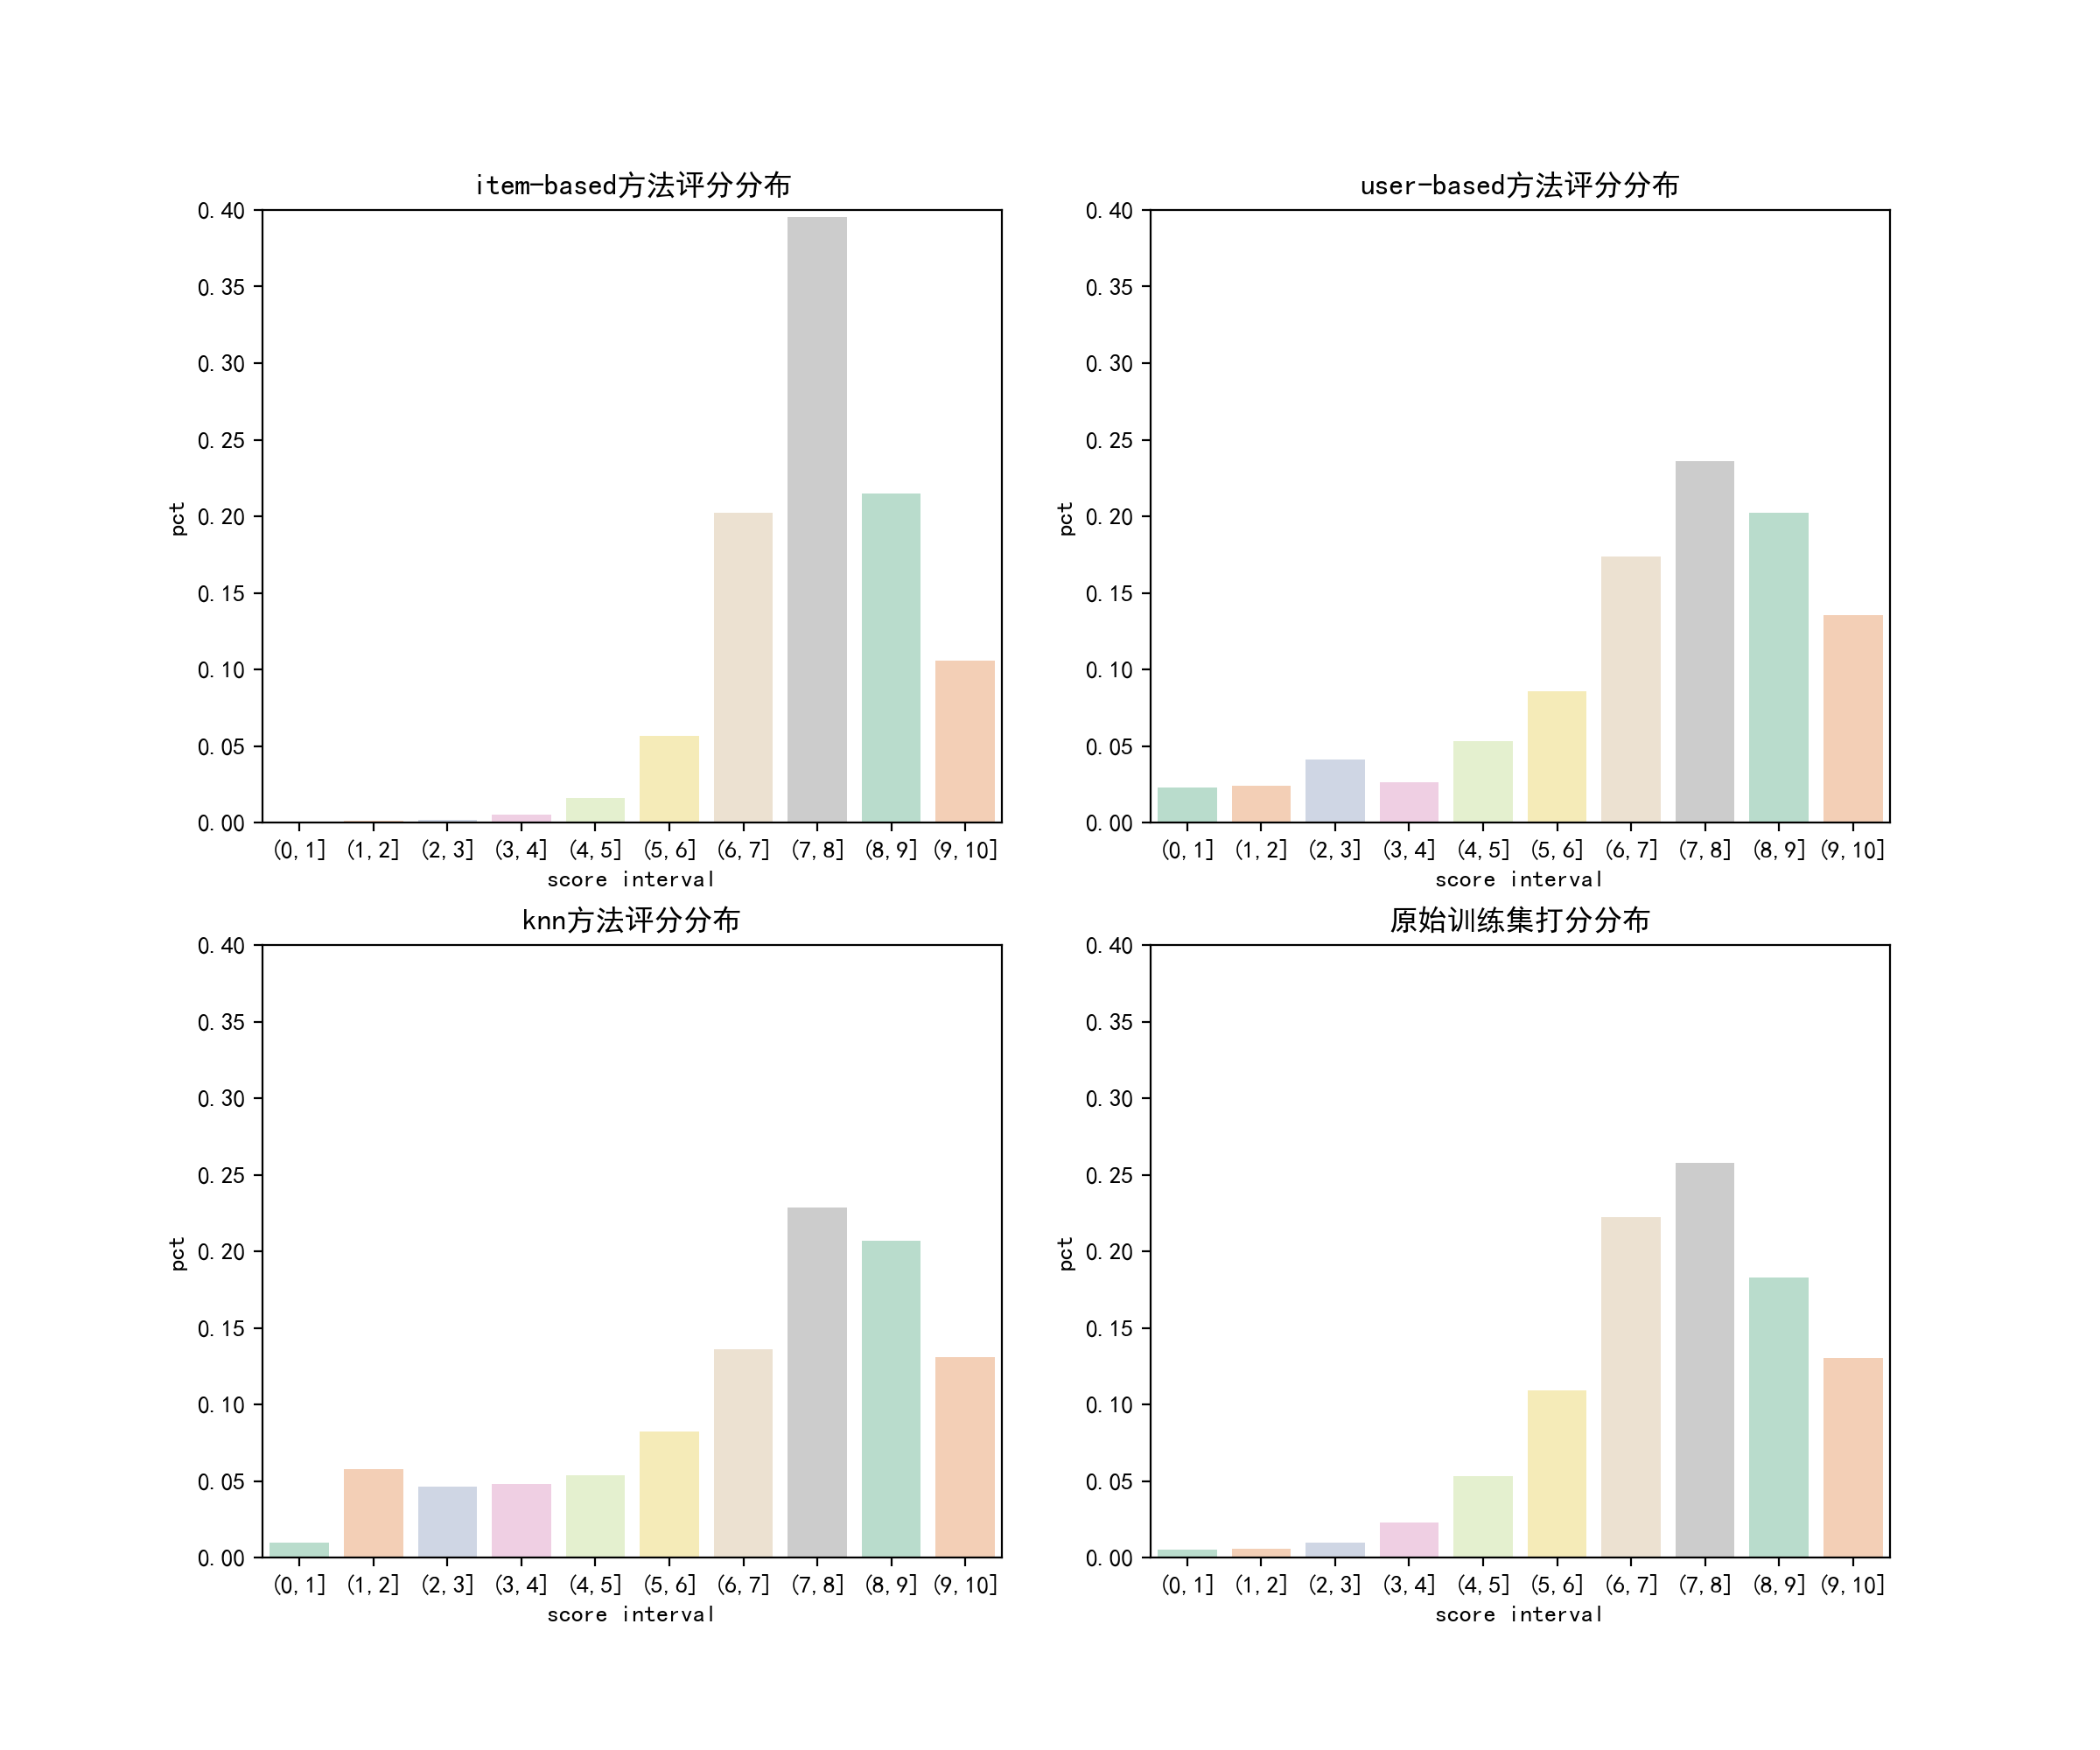
\includegraphics[height=12.0cm,width=16.0cm]{figure/pred_score.png}
      \caption{三种填充方法各自预测评分结果的分布情况}
      \label{fig: pred_score_distribution}
    \end{figure}

    表~\ref{tab:missing_imputation_results_3}是用KNN及两种基于领域的方法对样本得分填充后,四种召回算法在测试集上的效果对比。
    % Table generated by Excel2LaTeX from sheet 'imputation'
    \begin{table}[htbp]
      \centering
      \caption{三种缺失填充方法结果对比}
      %\textbf{表4.11}~~三种填充方法比较
      \resizebox{\textwidth}{!}{
        \begin{tabular}{rlrrrrrrrr}
          \toprule
          &      & \multicolumn{4}{c}{K=10}  & \multicolumn{4}{c}{K=20} \\
          \cmidrule{3-10}    \multicolumn{1}{l}{Algorithm} & Imputation & \multicolumn{1}{l}{Recall} & \multicolumn{1}{l}{Precision} & \multicolumn{1}{l}{Hit\_rate} & \multicolumn{1}{l}{Coverage} & \multicolumn{1}{l}{Recall} & \multicolumn{1}{l}{Precision} & \multicolumn{1}{l}{Hit\_rate} & \multicolumn{1}{l}{Coverage} \\
          \midrule
          \multicolumn{1}{l}{Item\_CF} & none & 2.148\% & 10.394\% & 44.700\% & 13.107\% & 3.778\% & 9.190\% & 55.744\% & 18.386\% \\
          & knn  & 2.272\% & \textbf{10.947\%} & 45.546\% & \textbf{13.572\%} & 3.981\% & \textbf{9.633\%} & 57.638\% & \textbf{20.771\%} \\
          & user & 2.244\% & 10.842\% & 45.546\% & 13.317\% & 3.931\% & 9.535\% & 56.711\% & 20.441\% \\
          & item & \textbf{2.284\%} & 10.840\% & \textbf{46.030\%} & 13.182\% & \textbf{4.044\%} & 9.618\% & \textbf{58.847\%} & 19.811\% \\
          \multicolumn{1}{l}{Item\_related} & none & 1.466\% & 7.247\% & 35.953\% & 22.615\% & 2.656\% & 6.770\% & 48.609\% & 27.070\% \\
          & knn  & 1.569\% & \textbf{7.728\%} & 38.210\% & 22.451\% & 2.807\% & 7.110\% & 49.980\% & 26.785\% \\
          & user & 1.541\% & 7.609\% & 37.565\% & 22.376\% & 2.817\% & \textbf{7.163\%} & 50.181\% & 26.920\% \\
          & item & \textbf{1.585\%} & 7.648\% & \textbf{38.613\%} & \textbf{22.466\%} & \textbf{2.866\%} & 7.108\% & \textbf{51.270\%} & \textbf{26.965\%} \\
          \multicolumn{1}{l}{gender+age} & none & 2.036\% & 9.177\% & 41.999\% & 3.824\% & 3.641\% & 8.230\% & 52.358\% & 5.324\% \\
          & knn  & \textbf{2.104\%} & \textbf{9.482\%} & \textbf{42.805\%} & \textbf{3.839\%} & \textbf{3.715\%} & \textbf{8.378\%} & 53.446\% & \textbf{5.849\%} \\
          & user & 2.093\% & 9.434\% & 42.523\% & 3.719\% & 3.665\% & 8.267\% & 52.842\% & 5.774\% \\
          & item & 2.075\% & 9.348\% & 42.563\% & 3.764\% & 3.684\% & 8.306\% & \textbf{53.567\%} & 5.849\% \\
          \multicolumn{1}{l}{Item\_similarity} & none & 2.438\% & 11.002\% & 48.408\% & 4.874\% & 4.350\% & 9.866\% & 58.081\% & 5.549\% \\
          & knn  & 2.462\% & 11.106\% & 48.811\% & \textbf{4.769\%} & 4.326\% & 9.796\% & 59.008\% & \textbf{5.579\%} \\
          & user & 2.455\% & 11.072\% & 48.771\% & 4.784\% & \textbf{4.352\%} & 9.849\% & 59.008\% & 5.564\% \\
          & item & \textbf{2.499\%} & \textbf{11.256\%} & \textbf{49.496\%} & 4.694\% & 4.348\% & \textbf{9.815\%} & \textbf{58.726\%} & 5.534\% \\
          \bottomrule
      \end{tabular}}%
      \label{tab:missing_imputation_results_3}%
    \end{table}%

    从结果上看,三种填充方法均对召回算法的结果有改善。具体地,knn方法对人口统计召回的提升效果比较好,基于物品邻域的评分预测对剩余的三种召回算法提升较大,而基于用户邻域的评分预测方法相对上述两种方法效果不是那么显著。

  \section{隐反馈特征的利用}
  前面实验中设置样本标签的方法是为my\_score字段设定一个阈值,打分高于阈值的样本为正样本,反之为负样本,阈值初设为8分。这样做只利用了用户打分这一显式反馈特征,没有充分利用数据集中其他一些与“用户是否喜欢该动漫”有联系的隐式反馈特征,而综合考虑隐反馈特征和显反馈特征来决定样本标签理应会使得推荐效果更好。本节下面的实验考虑如下两个隐反馈特征:my\_watched\_episodes(用户观看的集数)和my\_status(用户观看状态)。
    \subsection{结合观看集数设置样本标签}
    对某个训练样本,若用户在打分时观看的集数占该动漫总集数的比例越大,可以认为其打分信息可信程度越高。因此在设置样本标签时可以在原有的打分阈值基础上加入一个新条件,即:用户观看集数/动漫总集数的比例大小,并同样给定一个阈值$ratio$:
    \begin{equation}
    \label{ratio}
    y=\begin{cases}
    1, & \text{my\_score}\geq 8\;\;\textbf{and}\;\;\frac{\text{my\_watched\_episodes}}{\text{episodes}}\geq ratio \\
    0, & \textbf{else}
    \end{cases}
    \end{equation}

    原始数据集中存在少量的动漫的episodes=0。若要用~\ref{ratio}构造样本,分母不能为零,因此要对这部分的数据进行缺失填充。填充的方法是用训练集中所有用户看过该动漫的最长集数来作为总集数的估计。表~\ref{tab:watched_ratio_results}是结合了观看集数比例设置样本标签后各组召回算法的效果,以及最后xgb精排后的结果。
    % Table generated by Excel2LaTeX from sheet 'watched'
    \begin{table}[htbp]
      \centering
      \caption{结合用户观看集数比例构造标签后的推荐结果}
      %\textbf{表4.12}~~考虑用户观看集数比例后的推荐效果
      \resizebox{\textwidth}{!}{
        \begin{tabular}{rlrrrr}
          \toprule
          \multicolumn{1}{l}{ratio\_threshold} & Algorithm & \multicolumn{1}{l}{Recall} & \multicolumn{1}{l}{Precision} & \multicolumn{1}{l}{Hit\;rate} & \multicolumn{1}{l}{Coverage} \\
          \midrule
          0    & \textbf{gender+age} & \textbf{3.641\%} & \textbf{8.230\%} & \textbf{52.358\%} & \textbf{5.324\%} \\
          0.5  & gender+age & 3.595\% & 8.126\% & 51.794\% & 5.339\% \\
          0.6  & gender+age & 3.591\% & 8.118\% & 51.673\% & 5.339\% \\
          0.7  & gender+age & 3.580\% & 8.092\% & 51.632\% & 5.339\% \\
          0.8  & gender+age & 3.568\% & 8.066\% & 51.552\% & 5.354\% \\
          0    & \textbf{Item-related} & \textbf{1.466\%} & \textbf{7.247\%} & \textbf{35.953\%} & \textbf{22.615\%} \\
          0.5  & Item-related & 1.543\% & 7.657\% & 37.525\% & 22.660\% \\
          0.6  & Item-related & 1.556\% & 7.724\% & 37.888\% & 22.466\% \\
          0.7  & Item-related & 1.543\% & 7.662\% & 37.646\% & 22.555\% \\
          0.8  & Item-related & 1.554\% & 7.722\% & 38.170\% & 22.376\% \\
          0    & \textbf{Item-CF} & \textbf{3.778\%} & \textbf{9.190\%} & \textbf{55.744\%} & \textbf{18.386\%} \\
          0.5  & Item-CF & 3.739\% & 9.104\% & 55.542\% & 21.056\% \\
          0.6  & Item-CF & 3.751\% & 9.133\% & 55.462\% & 21.101\% \\
          0.7  & Item-CF & 3.744\% & 9.118\% & 55.421\% & 21.131\% \\
          0.8  & Item-CF & 3.730\% & 9.084\% & 55.139\% & 21.251\% \\
          0    & \textbf{Item-similarity} & \textbf{4.208\%} & \textbf{9.498\%} & \textbf{57.517\%} & \textbf{5.624\%} \\
          0.5  & Item-similarity & 4.319\% & 9.800\% & 58.525\% & 5.759\% \\
          0.6  & Item-similarity & 4.320\% & 9.805\% & 58.565\% & 5.729\% \\
          0.7  & Item-similarity & 4.316\% & 9.795\% & 58.565\% & 5.729\% \\
          0.8  & Item-similarity & 4.331\% & 9.830\% & 58.525\% & 5.729\% \\
          0    & \textbf{xgboost} & \textbf{7.469\%} & \textbf{11.203\%} & \textbf{77.872\%} & \textbf{21.296\%} \\
          0.5  & xgboost & 7.587\% & 11.392\% & 77.711\% & 24.280\% \\
          0.6  & xgboost & 7.575\% & 11.388\% & 77.348\% & 23.635\% \\
          0.7  & xgboost & 7.566\% & 11.361\% & 77.872\% & 23.410\% \\
          0.8  & xgboost & 7.549\% & 11.336\% & 77.227\% & 23.815\% \\
          \bottomrule
      \end{tabular}}%
      \label{tab:watched_ratio_results}%
    \end{table}%

    从表~\ref{tab:watched_ratio_results}可以得到:
    \begin{itemize}
      \item 设置了$ratio$阈值后,Item-related召回和Item-similarity召回的结果都有比较明显的提升;人口统计召回和Item-based CF召回效果略微下降;
      \item 设置了$ratio$阈值后,xgboost重排效果也有了明显提升。相对来说,ratio阈值较低时,重排后的结果会更好一些。
    \end{itemize}

    因此将特征my\_watched\_episodes纳入样本标签构造的规则中是有显著作用的。

    \subsection{结合观看状态来设置样本标签}
    表~\ref{tab:status_score_distribution}显示了不同的my\_status对应的打分分布是有显著差异的,因此统一的设置打分阈值并不是十分的合理,样本不同的my\_status取值$i$应当对应一个不同的打分阈值$t_i$。另一方面,各状态样本所占比例也不一样,显然对于样本比例大的状态,其阈值选取对结果的影响也越大。下面是对各状态的阈值变化对应推荐效果变化的探索分析,类似于grid-search(更多结果详见附录A):

    \begin{enumerate}
      \item $my\_status=2$:令$t_2\in\{7,8,9\}$,其余状态阈值为:$t_1\in\{7,8,9\},\;\;t_3\in\{7,8\},\;\;t_4=8$,共可比较六组实验结果,表~\ref{tab:status=2}是其中一组的结果(阈值分别为$t_1=8,\;t_3=8,\;t_4=8$)。可以看出:$t_2=8$时的最终推荐效果,要显著优于$t_2=7\;\text{or}\;9$时的效果。
      % Table generated by Excel2LaTeX from sheet 'status=2'
      \begin{table}[htbp]
        \centering
        \caption{my\_status=2对应不同阈值下的推荐结果}
        %\textbf{表4.13}~~ my\_status=2的阈值变化结果
        \resizebox{\textwidth}{!}{
          \begin{tabular}{rlrrrr}
            \toprule
            \multicolumn{1}{l}{threshold} & Algorithm & \multicolumn{1}{l}{Recall} & \multicolumn{1}{l}{Precision} & \multicolumn{1}{l}{Hit\;rate} & \multicolumn{1}{l}{Coverage} \\
            \midrule
            7    & gender+age & 3.510\% & 7.932\% & 50.988\% & 5.369\% \\
            8    & gender+age & 3.641\% & 8.230\% & 52.358\% & 5.324\% \\
            9    & gender+age & 3.722\% & 8.417\% & 54.373\% & 5.339\% \\
            7    & Item-related & 1.489\% & 7.303\% & 36.638\% & 22.705\% \\
            8    & Item-related & 1.466\% & 7.247\% & 35.953\% & 22.615\% \\
            9    & Item-related & 1.418\% & 7.302\% & 34.865\% & 22.271\% \\
            7    & Item-CF & 3.577\% & 8.686\% & 53.648\% & 21.371\% \\
            8    & Item-CF & 3.778\% & 9.190\% & 55.744\% & 18.386\% \\
            9    & Item-CF & 3.770\% & 9.224\% & 58.565\% & 26.770\% \\
            7    & Item-similarity & 4.423\% & 10.022\% & 58.888\% & 5.474\% \\
            8    & Item-similarity & 4.208\% & 9.498\% & 57.517\% & 5.624\% \\
            9    & Item-similarity & 4.072\% & 9.264\% & 56.993\% & 5.759\% \\
            7    & xgboost & 7.340\% & 11.021\% & 77.106\% & 22.735\% \\
            8    & \textbf{xgboost} & \textbf{7.469\%} & \textbf{11.203\%} & \textbf{77.872\%} & \textbf{21.296\%} \\
            9    & xgboost & 7.385\% & 11.092\% & 77.194\% & 26.110\% \\
            \bottomrule
        \end{tabular}}%
        \label{tab:status=2}%
      \end{table}%
      
      \item $my\_status=1$:令$t_1\in\{7,8,9\}$,其余状态阈值为:$t_3\in\{7,8\},t_2=t_4=8$,从表~\ref{tab:status=1}可以看出:$t_1=9$时的最终推荐效果略优
      % Table generated by Excel2LaTeX from sheet 'status=1'
      \begin{table}[htbp]
        \centering
        \caption{my\_status=1对应不同阈值下的推荐结果}
        %\textbf{表4.14}~~my\_status=1的阈值变化结果
        \resizebox{\textwidth}{!}{
          \begin{tabular}{rlrrrr}
            \toprule
            &      & \multicolumn{1}{l}{$t_3=8$} &      & \multicolumn{1}{l}{$t_3=7$} &  \\
            \cmidrule{3-6}    \multicolumn{1}{l}{threshold} & Algorithm & \multicolumn{1}{l}{Recall} & \multicolumn{1}{l}{Precision} & \multicolumn{1}{l}{Recall} & \multicolumn{1}{l}{Precision} \\
            \midrule
            7    & gender+age & 3.642\% & 8.234\% & 3.647\% & 8.244\% \\
            8    & gender+age & 3.641\% & 8.230\% & 3.641\% & 8.230\% \\
            9    & gender+age & 3.624\% & 8.193\% & 3.622\% & 8.188\% \\
            7    & Item-related & 1.466\% & 7.244\% & 1.477\% & 7.285\% \\
            8    & Item-related & 1.466\% & 7.247\% & 1.470\% & 7.258\% \\
            9    & Item-related & 1.474\% & 7.296\% & 1.469\% & 7.258\% \\
            7    & Item-CF & 3.772\% & 9.170\% & 3.766\% & 9.153\% \\
            8    & Item-CF & 3.778\% & 9.190\% & 3.736\% & 9.082\% \\
            9    & Item-CF & 3.708\% & 9.017\% & 3.714\% & 9.030\% \\
            7    & Item-similarity & 4.323\% & 9.804\% & 4.370\% & 9.909\% \\
            8    & Item-similarity & 4.208\% & 9.498\% & 4.361\% & 9.890\% \\
            9    & Item-similarity & 4.332\% & 9.829\% & 4.341\% & 9.848\% \\
            7    & xgboost & 7.453\% & 11.181\% & 7.437\% & 11.167\% \\
            8    & xgboost & 7.469\% & 11.203\% & 7.447\% & 11.182\% \\
            9    & xgboost & \textbf{7.523\%} & \textbf{11.296\%} & \textbf{7.533\%} & \textbf{11.311\%} \\
            \bottomrule
        \end{tabular}}%
        \label{tab:status=1}%
      \end{table}%
      
      \item $my\_status=4$:令$t_4\in\{5,6,7,8\}$,其余状态阈值为:$t_1=9,\;t_2=t_3=8$。从表~\ref{tab:status=4}可以看出:$t_4\geq 6$时的模型效果都优于原始模型的效果,而当$t_4\leq 5$后,有一个显著的下滑,因此适当的阈值选取应该在6分及以上。
      % Table generated by Excel2LaTeX from sheet 'status=4'
      \begin{table}[htbp]
        \centering
        \caption{my\_status=4对应不同阈值下的推荐结果}
        %\textbf{表4.15}~~my\_status=4的阈值变化结果
        \resizebox{\textwidth}{!}{
          \begin{tabular}{rlrrrr}
            \toprule
            \multicolumn{1}{l}{threshold} & Algorithm & \multicolumn{1}{l}{Recall} & \multicolumn{1}{l}{Precision} & \multicolumn{1}{l}{Hit\;rate} & \multicolumn{1}{l}{Coverage} \\
            \midrule
            5    & gender+age & 3.640\% & 8.228\% & 52.559\% & 5.354\% \\
            6    & gender+age & 3.639\% & 8.226\% & 52.439\% & 5.324\% \\
            7    & gender+age & 3.628\% & 8.201\% & 52.358\% & 5.309\% \\
            8    & gender+age & 3.624\% & 8.193\% & 52.277\% & 5.309\% \\
            5    & Item-related & 1.478\% & 7.293\% & 36.518\% & 22.406\% \\
            6    & Item-related & 1.469\% & 7.262\% & 36.195\% & 22.645\% \\
            7    & Item-related & 1.477\% & 7.305\% & 36.195\% & 22.481\% \\
            8    & Item-related & 1.474\% & 7.296\% & 36.034\% & 22.451\% \\
            5    & Item-CF & 3.726\% & 9.057\% & 55.341\% & 20.711\% \\
            6    & Item-CF & 3.710\% & 9.020\% & 55.099\% & 21.071\% \\
            7    & Item-CF & 3.719\% & 9.041\% & 55.462\% & 21.251\% \\
            8    & Item-CF & 3.708\% & 9.017\% & 55.139\% & 21.326\% \\
            5    & Item-similarity & 4.344\% & 9.855\% & 58.807\% & 5.654\% \\
            6    & Item-similarity & 4.340\% & 9.847\% & 58.605\% & 5.654\% \\
            7    & Item-similarity & 4.332\% & 9.829\% & 58.605\% & 5.654\% \\
            8    & Item-similarity & 4.332\% & 9.829\% & 58.726\% & 5.714\% \\
            5    & xgboost & 7.457\% & 11.197\% & 78.517\% & 22.076\% \\
            6    & xgboost & 7.518\% & 11.290\% & 78.033\% & 22.780\% \\
            7    & xgboost & 7.531\% & 11.309\% & 78.275\% & 22.211\% \\
            8    & xgboost & 7.523\% & 11.296\% & 77.993\% & 22.825\% \\
            \bottomrule
        \end{tabular}}%
        \label{tab:status=4}%
      \end{table}%
    \end{enumerate}

    综上,除了$my\_status=2$的阈值选取对各召回算法效果以及最终排序结果有比较明显的影响外,其他$my\_status$的阈值改变对结果的影响其实比较微弱。这很大程度上是因为样本特征$my\_status$取值极其不平衡,所以占据极大比例的状态2的阈值选取才是最关键的。但是如果数据集的组成有类似的隐式特征,同时类别比较均衡的时候,根据不同类设置不同阈值肯定会起到更明显的作用。		% 实验分析
%% !TEX root = ../thesis.tex

\chapter{实验分析}
\section{基本实验结果}
初次实验基于的数据集就是对全量用户随机采样5\%后根据日期划分而成的训练集和测试集,其中训练集基本只保留非零打分(my\_status=4除外)。对于根据这种规则划分得到的训练测试集,会出现“新用户”以及“新动漫”(下面用“新番”称谓)两种情况。新用户指的是在2017年6月30日之前没有过行为,或者是打分均为零的那些用户;新番指的就是首映日期在2017年6月30日以后的那些动漫。
\subsection{四种召回算法}
本实验采用的召回算法主要有四种,分别是Item-based CF召回,Item-related召回, 人口统计召回以及Item-similarity召回。其中Item-based CF召回属于协同过滤算法,人口统计召回属于基于规则的推荐,Item-similarity召回有点类似基于内容的推荐,而Item-related召回则是根据数据集自带特征的特点进行的关联推荐。下面分别简要介绍一下这四种算法的流程:
\subsubsection{Item-based CF}
这个在前面介绍协同过滤算法的时候已经提过了,这里用的就是这个经典的基于物品的协同过滤算法\cite{wang2006unifying}。下面是算法的伪代码:
\begin{algorithm}[htbp]
	\caption{Item-based CF}
	\KwIn{$u\in\tilde{U},\;W,\;I(u),\;S(u),\;K_1,\;K_2$}
	\KwOut{$R(u)$}
	$res=\{\},\;R(u)=[]$\;
	\If{$I(u)=\emptyset\;\;\textbf{or}\;\;S(u)=\emptyset$}{
		return $[]$\;}
	\For{$i \in I(u)$}{
		$cnt=0$\;
		\For{$j,w_j \in\;sort(W[i])$}{
			\If{$j \in S(u)$}{\textbf{continue}\;}
			$res[j]\leftarrow res[j]+w_j$\;
			$cnt\leftarrow cnt+1$\;
			\If{$cnt\geq K_1$}{\textbf{Break}\;}
		}
	}
	$R(u)=sort(res,K_2)$\;
	return $R(u)$\;
\end{algorithm}
符号说明:$\tilde{U}$是全体测试集用户;$W$是物品相似度矩阵;$I(u)$是用户$u$在训练集中喜欢的动漫集合;$S(u)$是用户$u$在训练集中观看过的动漫集合;$K_1,K_2$分别是选取的邻域大小以及最终召回的动漫个数;$R(u)$是最后为用户$u$召回的动漫集合。

\subsubsection{Item-related召回}
这是根据数据集Animelist的某一个特征进行的一种类似关联推荐的方法。具体地,在动漫信息数据集中有一列特征叫做related,里面存储了和这部动漫有所关联的动漫、漫画以及其相关联的方式。涉及到的关联方式主要有:
\begin{itemize}
	\item Adaptation:改编,占所有related key比例的30\%,但是通过
	Adaptation关联到的都是漫画,而漫画是不在我们数据集的包含范围内(我们推荐的目标局限于TV动画、OVA、Special、Movie等等,都是动画或是影视)
	\item Sequel/Prequel:续集/前传,这二者是一一对应的,占所有related key比例的28\%。通常动漫A的OVA会作为A的Sequel关联
	\item Parent story/Side story:父篇/番外,这二者也是一一对应的,占所有related key比例的15\%
\end{itemize}
其他的一些关联方法数量比较少,因此这种方法主要是根据Sequel、Prequel、Parent story和Side story这四种related methods来进行关联推荐。具体进行召回的方法是:对每个用户历史上喜欢的动漫按照打分从高到低排序,然后依次通过related方式关联到新的动漫(也可能没有关联),如果这部动漫没有被用户看过,那就进入召回列表。下面是伪代码:
\begin{algorithm}[htbp]
	\caption{Item-related Recall}
	\KwIn{$u\in\tilde{U},\;Re,\;I(u),\;S(u),\;K$}
	\KwOut{$R(u)$}
	\If{$I(u)=\emptyset\;\;\textbf{or}\;\;S(u)=\emptyset$}{return $\{\}$\;}
	$cnt=0$\;
	\For{$i \in sort(I(u))$}{
		\For{$j \in Re(i)$}{
			\If{$j\notin R(u)\;\;\textbf{and}\;\;j\neq[]\;\;\textbf{and}j\notin S(u)$}{
				$cnt\leftarrow cnt+1$\;
				$R(u)\leftarrow R(u)\cup \{j\}$\;
			}
			\If{$cnt\geq K$}{\textbf{Break}\;}
		}
		\If{$cnt\geq K$}{\textbf{Break}\;}
	}
\end{algorithm}

符号说明:基本与Item-based CF的符号一致,$Re(i)$是动漫$i$通过related
字段相关联的动漫集合;$sort(I(u))$是对用户$u$喜欢的动漫根据打分排序;$K$是最终召回的动漫数

\subsubsection{人口统计召回}
这个召回算法应该被划分为基于规则的推荐。在用户信息数据集User\_cleaned中,记录的都是关于每一个用户的一些固有属性特征,其中人口统计特征主要有gender(性别), location(地域)和birth\_date(出生日期)。人口统计学特征也可以用来帮助预测用户的兴趣,比方说:不同性别的用户所喜好的动漫一般有所不同,男性可能更喜欢热血、科幻向的,女性可能更喜欢清新、文艺向的;不同年龄层次的用户的偏好也会有所差异,年纪大的用户由于生活的沉淀,可能会更喜欢一些有内涵的动漫。由于数据集中的location字段非常多,取值参差不齐,同一个国家和地区也有许多不同的表示方法,比较难处理,所以本实验只选用了gender+age两个特征来进行人口统计学召回。

另一方面,人口统计召回也是解决用户冷启动的一种方法。如果对于测试集中的某个用户,其在训练集中没有喜欢的动漫,或是根本没有评过分,也就是$u\in\tilde{U},\;s.t.\;I(u)=\emptyset\;\;\textbf{or}\;\;S(u)=\emptyset$,那么上述两种算法都无法做出推荐。但是基于人口统计的召回就可以,因为即使是新用户,也存在年龄和性别,只要有年龄和性别,就可以根据训练集中同年龄段,同性别的其他用户所喜欢的动漫来给新用户做出推荐。

对于性别gender,数据集中可取值有Male, Female和Non-Binary,均保留。而对于年龄age,计算的方法是用训练集测试集的划分日期2017-06-30,减去用户的出生日期而得。由于是连续变量,因此再对其进行如下的分箱处理:
\begin{itemize}
	\item $age\in[11,19)$: Teenager
	\item $age\in[19,22)$: Youth
	\item $age\in[22,26)$: YouthAdult
	\item $age\in[26,30)$: Adult
	\item $age\in[30,50)$: MiddleAged
\end{itemize}
整个召回算法分为两个步骤:
\begin{enumerate}
	\item 第一步是生成训练集中不同(gender,age)值对所对应的热门动漫排序。具体地,首先对于每个可能的(gender,age)值对,统计训练集中每一部动漫在该性别年龄分组下的平均得分以及平均喜欢率(即label的均值);然后排除掉一部分过于小众的动漫,这里选择的方法是过滤掉样本记录数少于该性别年龄段总人数的20\%的动漫;最后对每部动漫的平均得分以及平均喜欢率分别作一个排名,然后取一个平均值作为该动漫在该(gender,age)分组下的最终排名。
	\item 第二步则是对测试集的每个用户,获取其性别与年龄,然后映射到第一步的返回集中找到其对应分组的topK部动漫,进行一定过滤后最终召回。
\end{enumerate}
下面是算法的伪代码:
\begin{algorithm}[htbp]
	\caption{Gender\&Age Ranking}
	\KwIn{$Train,\;gender,\;age$}
	\KwOut{$Ranking(gender,age)$}
	Get all the records in $Train$ given $gender$ and $age$, named $T_{g,a}$\;
	Caculate average score and label of $T_{g,a}$, grouped by each anime\_id\;
	Delete some anime\_id if the number of its samples is less than $20\%$ of the total users of $T_{g,a}$\;
	Caculate the final ranking for each anime\_id in $T_{g,a}$, that is:
	$$rank(anime\_id) = \left.\big(rank(avg\_score)+rank(avg\_label)\big)\middle/2\right.$$\;
	$Ranking(gender,age) = sort(\{anime\_id,rank(anime\_id)\})$\;
	return $Ranking(gender,age)$\;
\end{algorithm}

\begin{algorithm}[htbp]
	\caption{Gender\&Age Recall}
	\KwIn{$u\in\tilde{U},\;\mathcal{U},Ranking(gender,age)\;S(u),\;K$}
	\KwOut{$R(u)$}
	$R(u)=\{\}$\;
	$age\leftarrow \mathcal{U}(u)[age],\quad gender\leftarrow \mathcal{U}(u)[gender]$\;
	\eIf{$gender\neq$ 'Non-Binary'}{
		$Recall\_list\leftarrow Ranking(gender,age)$\;
		\For{$i \in Recall\_list$}{
			\If{$i \in S(u)$}{\textbf{Continue}\;}
			$R(u)\leftarrow R(u)\cup \{i\}$\;
			\If{$|R(u)|\geq K$}{\textbf{Break}\;}
		}
		return $R(u)$\;
	}{
		$Recall\_list_1\leftarrow Ranking('Male',age)$\;
		\For{$i \in Recall\_list_1$}{
			\If{$i \in S(u)$}{\textbf{Continue}\;}
			$R(u)\leftarrow R(u)\cup \{i\}$\;
			\If{$|R(u)|\geq K/2$}{\textbf{Break}\;}
		}
		$Recall\_list_2\leftarrow Ranking('FeMale',age)$
		\For{$i \in Recall\_list_2$}{
			\If{$i \in S(u)$}{\textbf{Continue}\;}
			$R(u)\leftarrow R(u)\cup \{i\}$\;
			\If{$|R(u)|\geq K$}{\textbf{Break}\;}
		}
	}
	return $R(u)$\;
\end{algorithm}

符号说明:$\mathcal{U}$是用户画像表,通过给定的$u$(用户id),可以获取他的性别和年龄;$Ranking(gender,age)$是第一步返回的中间结果,是不同性别和年龄分组下的TopAnime;$S(u)$是用户$u$在训练集中观看过的动漫集合;$K$是最终召回的动漫数。

\subsubsection{Item-similarity召回}
这个召回算法可以近似看成Content-based召回,主要是通过特征向量来计算物品与物品之间的相似度,然后根据用户在训练集中喜欢的动漫,来推荐与其相似的动漫。不过这种方法和Item-based CF比较相似,所以这里所做的改变是:只推荐new anime,即只为用户推荐在2017-06-30之后上映的动漫。因为这些new anime在训练集中肯定没有出现过,所以无论是Item-based CF还是人口统计召回都无法召回这些新动漫,Item-related召回方法因为是通过固有字段进行关联,所以可能会召回出新动漫,而Item-similarity召回则是完全专注于new anime的推荐,这也弥补了前面三种召回算法的不足之处。

具体地,物品间相似度的计算用的是普通的余弦相似度,每一部anime各自对应一个特征向量,特征向量的组成主要用到了动漫信息表中的genre(流派)、source(原作类型)以及部分rating(适宜人群),共20维的一个0-1向量。因为是召回新番,所以相似度的计算主要是计算旧番和新番之间的相似度,得到相似度之后,类比Item-based CF的方法就可以求得用户$u$对各个新番的喜好程度(相似度的累加),最后取前TopK个动漫作为召回结果。特别地,如果是新用户的话,就要先用人口统计召回的方法,获得新用户可能喜欢的old anime,然后再计算new anime的权重。下面是算法的伪代码:
\begin{algorithm}
	\caption{Item-similarity Recall}
	\KwIn{$u\in\tilde{U},\;W,\;I(u),\; GA(u),\;K_1,\;K_2$}
	\KwOut{$R(u)$}
	$res=\{\},\;R(u)=[]$\;
	\If{$I(u)=\emptyset$}{$I(u)\leftarrow GA(u)$\;}
	\For{$i \in I(u)$}{
		\For{$j,w_j \in\;sort(W[i])[:K_1]$}{
			$res[j]\leftarrow res[j]+w_j$\;
		}
	}
	$R(u)=sort(res,K_2)$\;
	return $R(u)$\;
\end{algorithm}
符号说明:$\tilde{U}$是全体测试集用户;$W$是新旧动漫余弦相似度矩阵;$I(u)$是用户$u$在训练集中喜欢的动漫集合;$GA(u)$是用户$u$的人口统计召回结果集;$K_1,K_2$分别是选取的邻域大小以及最终召回的动漫个数;$R(u)$是最后为用户$u$召回的动漫集合。

\subsection{召回结果比较}
首先先比较Item-based CF和Item-similarity Recall在邻域参数$K_1$的不同取值下的效果:
% Table generated by Excel2LaTeX from sheet 'Sheet1'
\begin{table}[htbp]
	\centering
	\caption{不同$K_1$取值下Item-based CF的效果}
	%\textbf{表4.1}~~不同$K_1$取值下Item-based CF的效果
	\begin{tabular}{rrrrrr}
		\toprule
		\multicolumn{1}{c}{Recall} & \multicolumn{1}{c}{Precision} & \multicolumn{1}{c}{Hit\;rate} & \multicolumn{1}{c}{Coverage} & \multicolumn{1}{c}{K1} & \multicolumn{1}{c}{K2} \\
		\midrule
		\textbf{2.148\%} & \textbf{10.394\%} & \textbf{44.700\%} & \textbf{13.107\%} & 5    & 10 \\
		2.093\% & 10.091\% & 41.798\% & 10.033\% & 10   & 10 \\
		2.066\% & 9.961\% & 40.911\% & 8.668\% & 15   & 10 \\
		2.015\% & 9.715\% & 40.427\% & 7.633\% & 20   & 10 \\
		1.986\% & 9.577\% & 40.508\% & 7.259\% & 25   & 10 \\
		\textbf{3.778\%} & \textbf{9.190\%} & \textbf{55.744\%} & \textbf{18.386\%} & 5    & 20 \\
		3.709\% & 8.972\% & 54.252\% & 15.102\% & 10   & 20 \\
		3.641\% & 8.791\% & 52.842\% & 13.362\% & 15   & 20 \\
		3.600\% & 8.680\% & 52.035\% & 11.938\% & 20   & 20 \\
		3.568\% & 8.603\% & 51.794\% & 11.338\% & 25   & 20 \\
		\bottomrule
	\end{tabular}%
	\label{tab:item-cf}%
\end{table}%

% Table generated by Excel2LaTeX from sheet 'Sheet1'
\begin{table}[htbp]
	\centering
	\caption{不同$K_1$取值下Item-similarity Recall的效果}
	%\textbf{表4.2}~~不同$K_1$取值下Item-similarity Recall的效果
	\begin{tabular}{rrrrrr}
		\toprule
		\multicolumn{1}{c}{Recall} & \multicolumn{1}{c}{Precision} & \multicolumn{1}{c}{Hit\;rate} & \multicolumn{1}{c}{Coverage} & \multicolumn{1}{c}{K1} & \multicolumn{1}{c}{K2} \\
		\midrule
		\textbf{2.437\%} & \textbf{11.002\%} & \textbf{48.408\%} & \textbf{4.874\%} & 5    & 10 \\
		2.445\% & 11.000\% & 47.561\% & 4.709\% & 10   & 10 \\
		2.372\% & 10.673\% & 47.037\% & 4.769\% & 15   & 10 \\
		2.298\% & 10.339\% & 46.352\% & 4.634\% & 20   & 10 \\
		2.262\% & 10.177\% & 45.425\% & 4.499\% & 25   & 10 \\
		\textbf{4.350\%} & \textbf{9.866\%} & \textbf{58.081\%} & \textbf{5.549\%} & 5    & 20 \\
		4.208\% & 9.498\% & 57.517\% & 5.624\% & 10   & 20 \\
		4.004\% & 9.022\% & 55.623\% & 5.729\% & 15   & 20 \\
		3.884\% & 8.738\% & 54.776\% & 5.789\% & 20   & 20 \\
		3.759\% & 8.456\% & 54.575\% & 5.609\% & 25   & 20 \\
		\bottomrule
	\end{tabular}%
	\label{tab:item-similarity}%
\end{table}%

从表~\ref{tab:item-cf}和表~\ref{tab:item-similarity}可以看出,不论是Item-based CF还是Item-similarity Recall,其算法效果与邻域参数$K_1$的大小呈负相关:$K_1$越小,最后的效果越好。因此在后面的实验中,均令这两种算法的$K_1=5$。

下面是四种召回算法在测试集上各自的效果对比,其中参数$K$表示最终召回的动漫数量,取值为$K\in\{10,20\}$。
% Table generated by Excel2LaTeX from sheet 'Sheet2'
\begin{table}[htbp]
	\centering
	\caption{四种召回算法各自在测试集上的表现}
	%\textbf{表4.3}~~四种召回算法各自在测试集上的表现
	\begin{tabular}{rlrrrr}
		\toprule
		\multicolumn{1}{l}{K} & Algorithm & \multicolumn{1}{l}{Recall} & \multicolumn{1}{l}{Precision} & \multicolumn{1}{l}{Hit\;rate} & \multicolumn{1}{l}{Coverage} \\
		\midrule
		10   & Item-CF & 2.148\% & 10.394\% & 44.700\% & 13.107\% \\
		& Item-related & 1.466\% & 7.247\% & 35.953\% & 22.615\% \\
		& gender+age & 2.036\% & 9.177\% & 41.999\% & 3.824\% \\
		& Item-similarity & 2.437\% & 11.002\% & 48.408\% & 4.874\% \\
		20   & Item-CF & 3.778\% & 9.190\% & 55.744\% & 18.386\% \\
		& Item-related & 2.656\% & 6.770\% & 48.609\% & 27.070\% \\
		& gender+age & 3.641\% & 8.230\% & 52.358\% & 5.324\% \\
		& Item-similarity & 4.350\% & 9.866\% & 58.081\% & 5.549\% \\
		\bottomrule
	\end{tabular}%
	\label{tab:recall}%
\end{table}%

从表~\ref{tab:recall}中可以得到如下结论:
\begin{itemize}
	\item 人口统计召回以及Item-similarity召回对应的覆盖率非常低,这是因为人口统计召回的都是同年龄同性别用户中的热门动漫,而新番原本占所有动漫的比例就比较低,所以覆盖率低是很正常的。
	\item 对于三种旧番召回算法,表现最好的应该是Item-based CF,这也说明协同过滤算法相比于基于规则的算法还有基于内容关联的算法性能要好。
	\item Item-related召回的表现是四种算法里最差的,因此最后占据的比例会比较小。不过该算法的覆盖率是最高的,可以增加推荐结果的多样性。
\end{itemize}

\subsection{用Xgboost进行精排}
得到了四组算法各自的召回结果后,还可以利用排序层的算法来对结果进行重排序,这可以看成是一个简单的机器学习二分类问题,具体地处理流程如下:
\begin{enumerate}
	\item 对于训练集,只保留user\_id、anime\_id和label三列(其余列均不进入模型),然后根据前面生成的用户画像表和动漫画像表,合并成一张最终训练表,并训练一个xgboost二分类模型
	\item 对于测试集,首先对测试集的每个user\_id,“捆绑”上四种召回算法各自的召回结果,换句话说,同一个user\_id会占据多行,每一行对应了某一种算法召回的一个anime\_id。然后同样地,合并上用户画像表和动漫画像表,形成最终的测试集,并利用训练好的xgboost模型进行预测打分
	\item 最后,对打分结果进行重排序。这里新番和旧番的排名分开计算,最终为每个用户返回分数最高的前10部新番和前20部旧番作为推荐结果列表。
\end{enumerate}
最终为每个用户生成的推荐列表大小$|R(u)|$是有一定依据的,表~\ref{tab:old_new_distribution}是测试集中平均每个用户观看的新番数量和旧番数量的四分位数分布情况:
% Table generated by Excel2LaTeX from sheet 'Sheet2'
\begin{table}[htbp]
	\centering
	\caption{测试集中用户观看的新番与旧番分布情况}
	%\textbf{表4.4}~~测试集中用户观看的新番与旧番分布情况
	\begin{tabular}{rrrr}
		\toprule
		\multicolumn{1}{l}{quantile} & \multicolumn{1}{l}{new\_anime\_count} & \multicolumn{1}{l}{old\_anime\_count} & \multicolumn{1}{l}{total\_anime\_count} \\
		\midrule
		mean & 17.18 & 45.60 & 62.78 \\
		std  & 23.22 & 84.97 & 98.59 \\
		25\% & 2    & 7    & 11 \\
		50\% & 9    & 19   & 32 \\
		75\% & 23   & 49   & 77 \\
		\bottomrule
	\end{tabular}%
	\label{tab:old_new_distribution}%
\end{table}%

而$|R(u)|$的大小正是依据了表~\ref{tab:old_new_distribution}中新旧番观看数量分布的中位数:新番召回10部,旧番召回20部。同时,根据表~\ref{tab:recall}中四种算法各自在测试集上的效果,给四种算法分配的K值分别是$20,10,20,20$,其中Item-related Recall的比例是最小的,因为它的效果相对是最差的。

二分类模型选用的是Xgboost集成学习算法\cite{chen2016xgboost},模型参数大多为默认值,一些手动设置的参数如下:
% Table generated by Excel2LaTeX from sheet 'Sheet1'
\begin{table}[htbp]
	\centering
	\caption{Xgboost参数设置}
	%\textbf{表4.5}~~Xgboost参数设置
	\resizebox{\textwidth}{!}{
		\begin{tabular}{rrrrrrrrrr}
			\multicolumn{1}{l}{Parameters} & \multicolumn{1}{l}{learning\_rate} & \multicolumn{1}{l}{n\_estimators} & \multicolumn{1}{l}{max\_depth} & \multicolumn{1}{l}{gamma} & \multicolumn{1}{l}{subsample} & \multicolumn{1}{l}{colsample\_bytree} & \multicolumn{1}{l}{reg\_alpha} & \multicolumn{1}{l}{reg\_lambda} & \multicolumn{1}{l}{random\_state} \\
			\midrule
			& 0.5  & 100  & 5    & 1    & 0.8  & 0.8  & 0    & 1    & 1001 \\
	\end{tabular}}%
	\label{tab:xgb_parameters}%
\end{table}%

而对召回结果进行重排序后,最终输出的推荐结果的评价指标如表~\ref{tab:xgb_result}所示:
% Table generated by Excel2LaTeX from sheet 'Sheet2'
\begin{table}[htbp]
	\centering
	\caption{Xgboost重排后的推荐结果}
	%\textbf{表4.6}~~Xgboost重排后的推荐结果
	\begin{tabular}{rrrr}
		\multicolumn{1}{l}{Recall} & \multicolumn{1}{l}{Precision} & \multicolumn{1}{l}{Hit\;rate} & \multicolumn{1}{l}{Coverage} \\
		\midrule
		7.469\% & 11.203\% & 77.872\% & 21.296\% \\
	\end{tabular}%
	\label{tab:xgb_result}%
\end{table}%

对比表~\ref{tab:recall}可以看出:经过排序后的推荐结果,无论是$Recall$, $Precision$还是$Hit\;rate$,都要比任意一种算法单独的效果要好很多。尤其是随着$K$的增加,$Precision$本应呈下降趋势,但是经过排序后的推荐结果的$Precision$不降反升。所以这个排序阶段可以很好地提高推荐系统的性能。



\section{抽样合理性讨论}
上一小节的实验主要比较了四种推荐召回算法各自的效果差异,并利用xgboost模型做了一个精排序,效果有显著提升。不过由于模型计算开销的问题,实验是基于采样后的数据集来做的,具体的方法是对全量用户随机抽样5\%。这一节讨论的是这个抽样的合理性,主要是通过全量、抽样以及增量训练三者的结果比较来看。
\subsection{增量学习的含义和特点}
增量学习(Incremental Learning)\cite{zhong2017survey}是指一个学习系统能不断地从新样本中学习新的知识,并能保存大部分以前已经学习到的知识。增量学习非常类似于人类自身的学习模式。其应用的主要场景有两个:一个是数据库非常大的情况,训练数据无法一次性装入计算机内存,这时候可以用增量学习的方法来训练模型,如大规模机器学习;另一个场景是针对流数据,随时间的变化不断变化。其主要特点有:
\begin{itemize}
	\item 可以从新数据中学习新知识。当新增数据时,只做关于新增数据引起的更新,同时保存以前学习到的大部分知识;
	\item 以前已经处理过的数据不需要重复处理
	\item 学习系统没有关于整个训练样本的先验知识
	\item —旦学习完成后训练观测样本被丢弃
\end{itemize}

用一个简单的例子来解释增量训练与全量训练相比的差别。假设现在有200条数据,用增量训练的方法,第一次训练150条,第二次训练50条。这个方法与全量训练直接拿200条数据训练得到的结果相比:增量训练在第二次训练50条数据的时候,前150条数据已经不存在于内存之中了,因此模型会更拟合于后面的新数据。不过后50条训练数据,是在前150条数据训练所得到的模型基础上进行训练的,因此会保留初始模型的一部分信息。所以如果要用增量训练,最好保证增量数据的质量均匀分布,防止把模型带偏。

Python中的xgboost api支持增量学习,根据官方文档的叙述,它提供的增量训练方法是将全量数据集分batch读入内存,迭代训练模型。每次训练好一个xgb模型后,下一轮迭代会从这个xgb模型的基础上出发,基于新一批的batch数据,保留树结构不变,刷新树节点的统计量和叶子节点的输出值。相关设置参数如下:
\begin{itemize}
	\item \mintinline{python}{process_type = update}: 从已有的模型出发,保留树的结构不变
	\item \mintinline{python}{updater = refresh}: 指定每轮迭代时树的更新方式。\mintinline{python}{refresh}表示利用新的数据,刷新原有树的内部节点的统计量。这里不会进行随机行采样。
	\item \mintinline{python}{refresh_leaf = True}: 关于\mintinline{python}{updater = refresh}的一个参数,设置为\mintinline{python}{True}时,不仅更新树的内部节点统计量,还会刷新叶子节点的输出值。
\end{itemize}

\subsection{增量训练的有效性}
为了检验xgb的incremental learning是否有效,我们把上一节实验所用到的90万行的抽样训练集,当做是假想的“全量数据集”,然后利用增量训练Xgboost的方法,逐步地训练分类模型,一并对抽样后的测试集进行排序预测,比较模型的效果。为了验证我们对用户抽样的合理性,在这里同样也对这个假想的“全量”训练集用户做一次5\%随机抽样,作为实验的对照组。

前文提过,增量训练最好能保证增量数据的质量均匀分布,因此下面的实验采用了三种不同的增量数据读入规则来比较相应的模型结果:
\begin{enumerate}
	\item 按默认数据集顺序读入。默认的训练数据集是按照anime\_id字段的取值大小升序排序的,换句话说,不同用户关于同一部动漫,在不同时间更新的状态、评分等行为样本,在训练集中是连续出现的;
	\item 按时间顺序读入。默认顺序会导致每轮更新时用到的数据只包含一小部分的anime信息。这一次把训练集按last\_update\_date字段取值升序排序,由远及近的分批读入;
	\item 随机顺序读入。最后则是把数据集完全随机打乱后再读入。
\end{enumerate}
按照三种顺序读入的增量训练模型结果如表~\ref{tab:incremental_results_3_orders}所示:
% Table generated by Excel2LaTeX from sheet 'incremental'
\begin{table}[htbp]
	\centering
	\caption{不同读入数据顺序下增量训练的结果}
	%\textbf{表4.7}~~不同读入数据顺序下增量训练的结果
	\resizebox{\textwidth}{!}{
		\begin{tabular}{rlrrrr}
			\toprule
			\multicolumn{1}{l}{Order} & Model & \multicolumn{1}{l}{Recall} & \multicolumn{1}{l}{Precision} & \multicolumn{1}{l}{Hit\_rate} & \multicolumn{1}{l}{Coverage} \\
			\midrule
			& Full amount training & \textbf{7.469\%} & \textbf{11.203\%} & \textbf{77.872\%} & \textbf{21.296\%} \\
			& Sampling training(5\%) & 7.039\% & 10.558\% & 76.622\% & 20.531\% \\
			\multicolumn{1}{l}{raw} & Incremental(first round) & 6.819\% & 10.228\% & 75.574\% & 22.256\% \\
			& Incremental(last round) & 7.127\% & 10.690\% & 76.824\% & 18.056\% \\
			\multicolumn{1}{l}{time} & Incremental(first round) & 7.203\% & 10.804\% & 76.179\% & 22.166\% \\
			& Incremental(last round) & 7.271\% & 10.906\% & 77.630\% & 17.622\% \\
			\multicolumn{1}{l}{random} & Incremental(first round) & 7.106\% & 10.658\% & 76.542\% & 22.091\% \\
			& Incremental(last round) & 7.323\% & 10.984\% & 77.227\% & 17.697\% \\
			\bottomrule
	\end{tabular}}%
	\label{tab:incremental_results_3_orders}%
\end{table}%

其中,"Full amount training"对应了“全量训练”,即用90万数据训练出的模型预测结果;"Sampling training"对应“抽样训练”,即再对90万数据中的用户进行$5\%$的抽样,所得的约5万数据来训练得到的模型结果;“Incremental”即是“增量训练”。三种方法的测试集均为全量测试,指的是用全量的90万数据来应用四种召回算法,然后为测试集用户生成召回样本集。可以看出:
\begin{itemize}
	\item 默认顺序下,从首轮到末轮,模型的预测效果有了较为明显的提高,更接近于全量数据下的表现,同时显著优于抽样数据下的表现。
	\item 时间顺序下,从首轮到末轮,增量模型的预测效果没有太大的变化,并且从首轮开始模型就已经很接近全量数据训练下的表现了,其效果仍然显著优于抽样的结果。
	\item 随机顺序下的表现和时间顺序下差不多。
	\item 从模型效果来看:全量$>$增量$>$抽样。
\end{itemize}

因此,Xgboost的incremental training api的的确确是起到了作用的,并且其增量训练的效果要优于抽样训练的结果。为了避免偶然因素,这里对90w数据中用户多做几次随机抽样并多次训练模型,比较其全量测试效果,如表~\ref{tab:multiple_sampling}所示:
% Table generated by Excel2LaTeX from sheet 'incremental'
\begin{table}[htbp]
	\centering
	\caption{对“全量”数据多次采样的结果}
	%\textbf{表4.8} 对“全量”数据多次采样的结果
	\begin{tabular}{rrrrr}
		\toprule
		\multicolumn{1}{l}{Times} & \multicolumn{1}{l}{Recall} & \multicolumn{1}{l}{Precision} & \multicolumn{1}{l}{Hit\;rate} & \multicolumn{1}{l}{Coverage} \\
		\midrule
		1    & 7.039\% & 10.558\% & 76.622\% & 20.531\% \\
		2    & 7.151\% & 10.726\% & 76.703\% & 22.705\% \\
		3    & 7.174\% & 10.761\% & 76.824\% & 21.341\% \\
		4    & 7.107\% & 10.660\% & 77.025\% & 21.641\% \\
		5    & 7.122\% & 10.682\% & 76.622\% & 22.271\% \\
		average & 7.119\% & 10.678\% & 76.759\% & 21.698\% \\
		full & \textbf{7.469\%} & \textbf{11.203\%} & \textbf{77.872\%} & \textbf{21.296\%} \\
		\bottomrule
	\end{tabular}%
	\label{tab:multiple_sampling}%
\end{table}%

从表~\ref{tab:multiple_sampling}中可以发现:这五次随机抽样的结果之间有些微的差异,不过共同的特点是他们基本上都比“全量”训练和增量训练的效果要差。

\subsection{全量数据抽样的合理性}
上一小节的实验验证了从预测表现来看,全量训练$>$增量训练$>$抽样训练。下面对原始的全量数据集(约1800万行)进行增量训练,比较其与抽样训练模型的全量预测表现,结果如表~\ref{tab:full_vs_sampling}。结果发现:我们抽样训练模型的结果要好于增量训练模型的预测结果。
% Table generated by Excel2LaTeX from sheet 'Sheet3'
\begin{table}[htbp]
	\centering
	\caption{全量数据的增量结果与$5\%$抽样的对比}
	%\textbf{表4.9}~~全量数据的增量结果与5\%抽样的对比
	\resizebox{\textwidth}{!}{
		\begin{tabular}{lrrrr}
			\toprule
			Model & \multicolumn{1}{l}{Recall} & \multicolumn{1}{l}{Precision} & \multicolumn{1}{l}{Hit\;rate} & \multicolumn{1}{l}{Coverage} \\
			\midrule
			Sampling training(5\%) & 7.358\% & 11.015\% & 76.736\% & 42.606\% \\
			Full Incremental(last round) & 7.195\% & 10.771\% & 76.402\% & 41.302\% \\
			\bottomrule
	\end{tabular}}%
	\label{tab:full_vs_sampling}%
\end{table}%

对比上一节把90万数据作为假想的“全量”数据,那时候的抽样结果是要明显差于增量结果的。而现在抽样的结果甚至优于增量训练结果。而之前已经证实了这个增量训练的确是起到了效果的,所以这应当可以说明:对于原始数据集1800万的大样本量来说,随机抽取5\%用户得到的这90万样本,可以比较好的代表总体样本,因而用这90万训练集得到的模型结果也比较可靠。更具体地,表~\ref{tab:liked_anime_quantile}是各个数据集中每个用户喜欢的动漫数的分布情况:
% Table generated by Excel2LaTeX from sheet 'Sheet3'
\begin{table}[htbp]
	\centering
	\caption{各数据集中用户喜好动漫数分布情况}
	%\textbf{表4.10}~~各数据集用户喜好动漫数分布情况
	\begin{tabular}{rrrrrrrr}
		\toprule
		\multicolumn{1}{l}{quantile} & \multicolumn{1}{l}{full} & \multicolumn{1}{l}{sampling} & 1    & 2    & 3    & 4    & 5 \\
		\midrule
		0.1  & 8    & 8    & 11   & 11.3 & 11   & 7    & 10.1 \\
		0.2  & 19   & 20   & 24.4 & 24   & 20   & 20.6 & 22 \\
		0.3  & 31   & 32   & 33   & 35   & 32   & 32   & 37 \\
		0.4  & 45   & 46   & 51   & 49   & 43   & 39.2 & 46.4 \\
		0.5  & 61   & 62   & 65   & 61   & 65.5 & 53   & 62.5 \\
		0.6  & 80   & 83   & 83.6 & 90.8 & 88.2 & 74.8 & 85 \\
		0.7  & 106  & 109  & 116  & 122.2 & 118.8 & 106.1 & 108.4 \\
		0.8  & 144  & 145  & 166.4 & 166.2 & 151.6 & 166.4 & 148 \\
		0.9  & 215  & 220  & 254  & 233.1 & 233.1 & 236.2 & 220.7 \\
		\bottomrule
	\end{tabular}%
	\label{tab:liked_anime_quantile}%
\end{table}%

其中,"full"表示全量1800万数据,"sampling"即是抽样的90万数据,而$1,2,3,4,5$分别对应表~\ref{tab:multiple_sampling}中五次抽样$5\%$所得的数据子集。通过观察很容易发现:我们的抽样数据集和全量数据集的各分位数分布非常接近,而二次抽样后的分布相对一次抽样来说,就有了明显的差异,这也从另一个角度说明了我们对全量数据进行抽样所得的结果和原始数据集相比仍保持着相似的分布,因此抽样训练得到的模型在全量测试集上的预测表现良好,可以用于解决全量召回结果排序的问题。

\section{数据稀疏解决}
表~\ref{tab:status_score_distribution}已经体现了数据稀疏这一特点,数据集中有许多的样本,它们的打分值my\_score=0,而在4.1节的实验中,是把这些$0$分样本基本都剔除出了训练集中,没有使用它们。这样会损失很多信息,这一节主要是对缺失得分进行填充。采用的方法有两种:基于K近邻的填充和基于邻域的评分预测填充。
\subsection{K近邻填充法}
K近邻(k-nearest neighbors, KNN)是一种非常基本的机器学习算法,其思想在日常生活中也是十分普遍。KNN既可以解决分类问题,又可以解决回归问题。具体地,在做分类问题时,采用多数投票法,即在训练集中,寻找和待遇测样本特征最相近的k个样本,把这k个样本中类别出现次数最多的那一类作为预测结果;在做回归问题时,采用平均法,同样是在训练集中,寻找和待遇测样本特征最相近的k个样本,然后把这k个样本的标签值求平均后作为回归的输出。

之前实验中用的训练集叫做$Train\_non\_zero$,顾名思义就是非零打分的样本集合(status=4的0分样本保留以外),而my\_status=1,2,3的零分样本合在一起叫做$Train\_zero$。现在我们的目标就是利用$Train\_non\_zero$作为训练集训练一个KNN的回归模型,然后对$Train\_zero$中的样本得分进行预测。在这里,我并没有选择把全部的$Train\_zero$都作为测试集,而是选出了其中,观看集数/总集数比例在$50\%$以上的那些样本。这是一个比较合理的处理,因为看的集数越多,最后打的分可信度会越高,对这些观看长度比例较高的样本进行预测比较有价值。

KNN回归模型的参数基本上用的是默认参数,其中\mintinline{python}{k=5}表示对每个样本寻找与其最近的5个训练样本,\mintinline{python}{weights='distance'}表示使用样本间欧氏距离作为权重,样本间距离越近就越重要。

\subsection{基于邻域的评分预测法}
这其实是评分推荐所使用的协同过滤算法,与TopN类似的,也可以分成基于用户的评分预测和基于物品的评分预测。
\begin{enumerate}
	\item 基于用户的评分预测:这种方法认为用户$u$对物品$i$的评分,可以参考用户$u$的平均打分,以及和用户$u$相似的其他用户对该物品的打分。具体地:
	\begin{equation}
	\hat{p}_{ui}=\bar{p}_u+\frac{\sum\limits_{v\in N(i)\cap B(u,k)}sim(u,v)(p_{vi}-\bar{p}_v)}{\sum\limits_{v\in N(i)\cap B(u,k)}sim(u,v)},
	\end{equation}
	其中,$\hat{p}_{ui}$是预测用户$u$对物品$i$的打分;$\bar{p}_u$是用户$u$的平均打分;$N(i)$是对物品有过评分的用户集合;$B(u,k)$是和用户$u$最相似的$k$个用户。
	
	用户间相似度计算用的是简单的余弦相似度,即每一个用户对应了一个评分向量,长度等于所有的动漫数,评过分的动漫其对应分量就等于具体的评分,没有评过分的动漫其对应分量位置等于零:
	\begin{equation}
	sim(u,v)=\frac{\sum\limits_{i\in I}p_{ui}\cdot p_{vi}}{\sqrt{\sum\limits_{i\in I}p_{ui}^2\cdot \sum\limits_{i\in I}p_{vi}^2}}.
	\end{equation}
	
	\item 基于物品的评分预测\cite{sarwar2001item}:这种方法认为用户$u$对物品$i$的评分,可以参考物品$i$的平均打分,以及用户对和物品$i$相似的其他物品的打分。具体地:
	\begin{equation}
	\hat{p}_{ui}=\bar{p}_i+\frac{\sum\limits_{j\in N(u)\cap B(i,k)}sim(i,j)(p_{uj}-\bar{p}_j)}{\sum\limits_{j\in N(u)\cap B(i,k)}sim(i,j)},
	\end{equation}
	其中,$\hat{p}_{ui}$是预测用户$u$对物品$i$的打分;$\bar{p}_i$是物品$i$的平均打分;$N(u)$是用户$u$评过分的物品集合;$B(i,k)$是和物品$i$最相似的$k$个物品。
	
	物品间相似度计算也用的是简单的余弦相似度,即每一个物品对应了一个评分向量,长度等于所有的用户数,某个用户对该物品评过分,则其对应分量就等于具体的评分,某用户没有对这部动漫评过分,则其对应分量位置等于零:
	\begin{equation}
	sim(i,j)=\frac{\sum\limits_{u\in U}p_{ui}\cdot p_{uj}}{\sqrt{\sum\limits_{u\in U}p_{ui}^2\cdot \sum\limits_{u\in U}p_{uj}^2}}.
	\end{equation}
\end{enumerate}

图~\ref{fig: pred_score_distribution}是这三种填充方法各自填充的评分结果分布图与原始训练数据集中的评分结果分布比较。可以看出:三种方法填充的评分分布情况与总体分布大体一致,其中基于用户邻域的方法和k近邻填充方法的评分预测分布较为平缓,而基于物品邻域的方法,其预测结果分数普遍较高。
\begin{figure}[htbp]
	\centering
	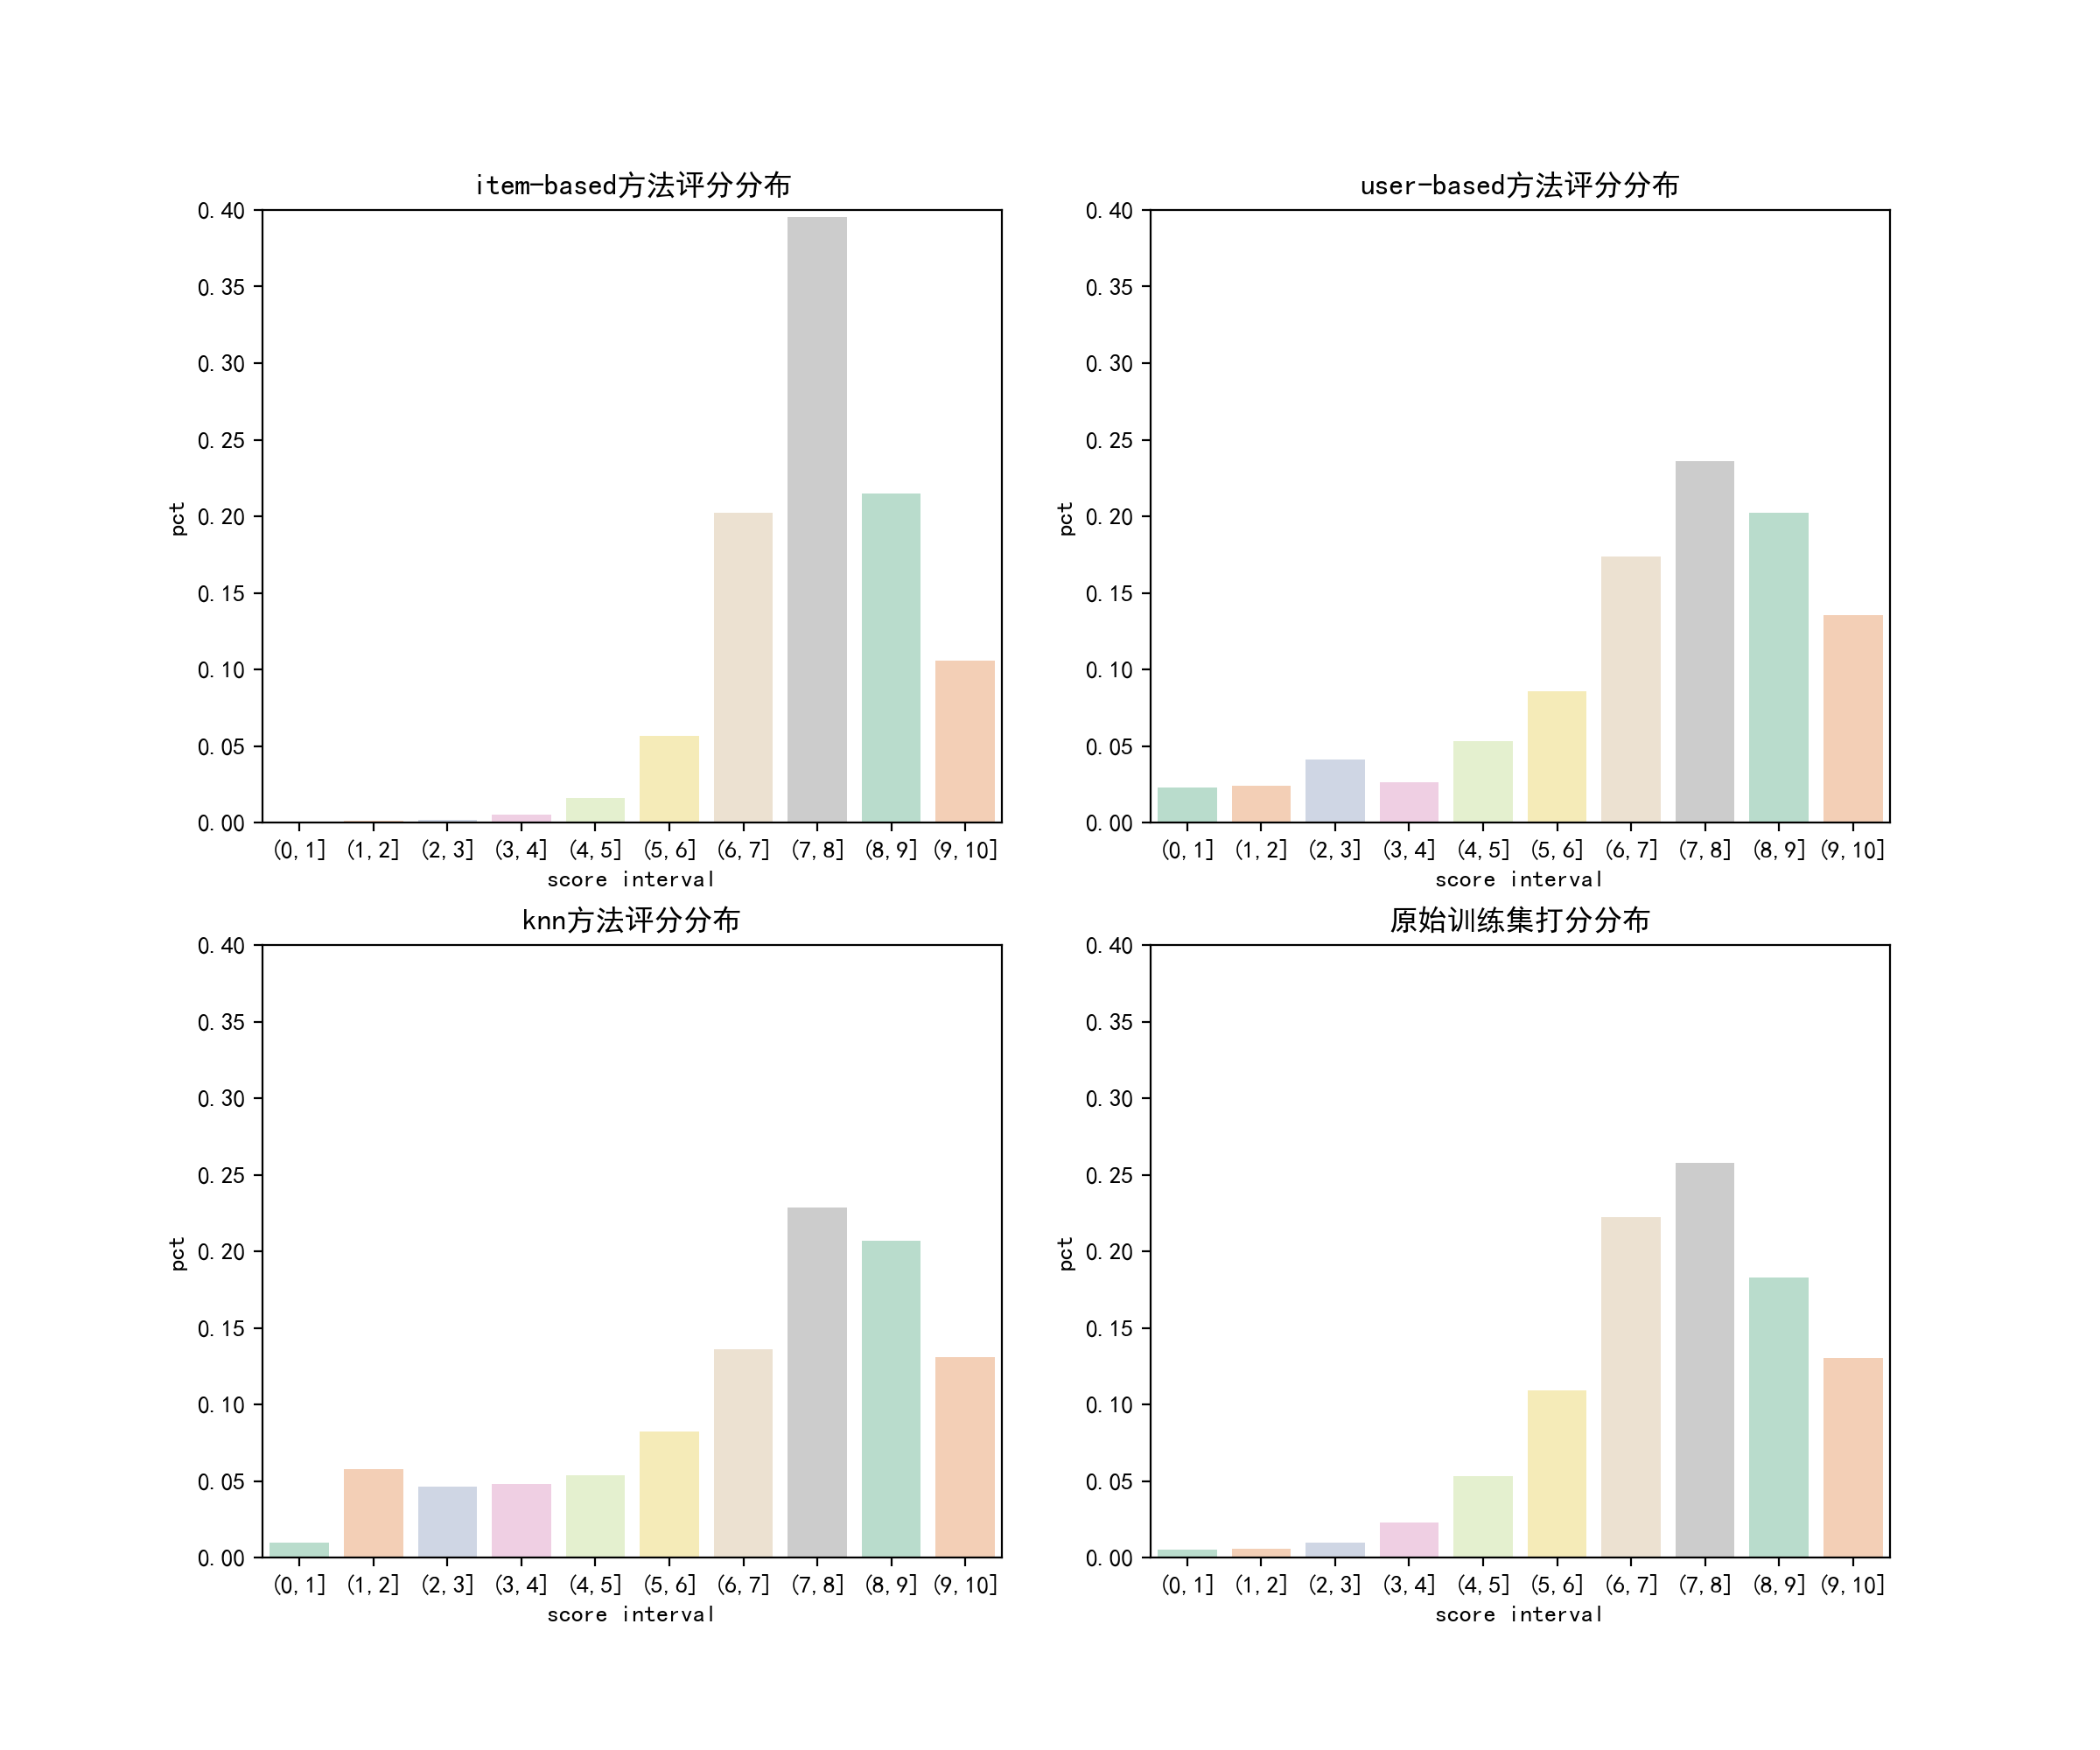
\includegraphics[height=12.0cm,width=16.0cm]{figure/pred_score.png}
	\caption{三种填充方法各自预测评分结果的分布情况}
	\label{fig: pred_score_distribution}
\end{figure}

表~\ref{tab:missing_imputation_results_3}是用KNN填充以及上述两种基于领域的方法对样本得分填充后,四种召回算法在测试集上的效果对比:
% Table generated by Excel2LaTeX from sheet 'imputation'
\begin{table}[htbp]
	\centering
	\caption{三种缺失填充方法结果对比}
	%\textbf{表4.11}~~三种填充方法比较
	\resizebox{\textwidth}{!}{
		\begin{tabular}{rlrrrrrrrr}
			\toprule
			&      & \multicolumn{4}{c}{K=10}  & \multicolumn{4}{c}{K=20} \\
			\cmidrule{3-10}    \multicolumn{1}{l}{Algorithm} & Imputation & \multicolumn{1}{l}{Recall} & \multicolumn{1}{l}{Precision} & \multicolumn{1}{l}{Hit\_rate} & \multicolumn{1}{l}{Coverage} & \multicolumn{1}{l}{Recall} & \multicolumn{1}{l}{Precision} & \multicolumn{1}{l}{Hit\_rate} & \multicolumn{1}{l}{Coverage} \\
			\midrule
			\multicolumn{1}{l}{Item\_CF} & none & 2.148\% & 10.394\% & 44.700\% & 13.107\% & 3.778\% & 9.190\% & 55.744\% & 18.386\% \\
			& knn  & 2.272\% & \textbf{10.947\%} & 45.546\% & \textbf{13.572\%} & 3.981\% & \textbf{9.633\%} & 57.638\% & \textbf{20.771\%} \\
			& user & 2.244\% & 10.842\% & 45.546\% & 13.317\% & 3.931\% & 9.535\% & 56.711\% & 20.441\% \\
			& item & \textbf{2.284\%} & 10.840\% & \textbf{46.030\%} & 13.182\% & \textbf{4.044\%} & 9.618\% & \textbf{58.847\%} & 19.811\% \\
			\multicolumn{1}{l}{Item\_related} & none & 1.466\% & 7.247\% & 35.953\% & 22.615\% & 2.656\% & 6.770\% & 48.609\% & 27.070\% \\
			& knn  & 1.569\% & \textbf{7.728\%} & 38.210\% & 22.451\% & 2.807\% & 7.110\% & 49.980\% & 26.785\% \\
			& user & 1.541\% & 7.609\% & 37.565\% & 22.376\% & 2.817\% & \textbf{7.163\%} & 50.181\% & 26.920\% \\
			& item & \textbf{1.585\%} & 7.648\% & \textbf{38.613\%} & \textbf{22.466\%} & \textbf{2.866\%} & 7.108\% & \textbf{51.270\%} & \textbf{26.965\%} \\
			\multicolumn{1}{l}{gender+age} & none & 2.036\% & 9.177\% & 41.999\% & 3.824\% & 3.641\% & 8.230\% & 52.358\% & 5.324\% \\
			& knn  & \textbf{2.104\%} & \textbf{9.482\%} & \textbf{42.805\%} & \textbf{3.839\%} & \textbf{3.715\%} & \textbf{8.378\%} & 53.446\% & \textbf{5.849\%} \\
			& user & 2.093\% & 9.434\% & 42.523\% & 3.719\% & 3.665\% & 8.267\% & 52.842\% & 5.774\% \\
			& item & 2.075\% & 9.348\% & 42.563\% & 3.764\% & 3.684\% & 8.306\% & \textbf{53.567\%} & 5.849\% \\
			\multicolumn{1}{l}{Item\_similarity} & none & 2.438\% & 11.002\% & 48.408\% & 4.874\% & 4.350\% & 9.866\% & 58.081\% & 5.549\% \\
			& knn  & 2.462\% & 11.106\% & 48.811\% & \textbf{4.769\%} & 4.326\% & 9.796\% & 59.008\% & \textbf{5.579\%} \\
			& user & 2.455\% & 11.072\% & 48.771\% & 4.784\% & \textbf{4.352\%} & 9.849\% & 59.008\% & 5.564\% \\
			& item & \textbf{2.499\%} & \textbf{11.256\%} & \textbf{49.496\%} & 4.694\% & 4.348\% & \textbf{9.815\%} & \textbf{58.726\%} & 5.534\% \\
			\bottomrule
	\end{tabular}}%
	\label{tab:missing_imputation_results_3}%
\end{table}%

从结果上看,三种填充方法都对召回算法的结果有改善。具体地,knn方法对人口统计召回的提升效果比较好,基于物品邻域的评分预测对剩余的三种召回算法提升较大,而基于用户邻域的评分预测方法相对上述两种方法效果不是那么显著。

\section{隐反馈特征的利用}
在第3.3节正负样本构造中,提到了怎样设置训练集和测试集的样本标签,当时的做法是为my\_score特征统一给定一个阈值,打分高于阈值的样本标签$y=1$,打分低于阈值的样本标签$y=0$,阈值的设定等于8分。但是这么做的话,数据集中其他一些与“用户是否喜欢该动漫”有联系的隐反馈特征就没有用上,因此综合考虑隐反馈特征和显反馈特征(打分)来决定样本标签应该会使得推荐效果更好。本节考虑如下两个隐反馈特征:my\_watched\_episodes(用户观看的集数)和my\_status(用户观看状态)。
\subsection{结合观看集数来设置样本标签}
对于训练集中的某一个样本,如果用户在打分时所观看的集数占该动漫总集数的比例越大,理应认为其对应的打分信息的可信程度越高,因此在设置样本标签时可以在原有的my\_score阈值基础上引入一个新的条件,即:用户观看集数/动漫总集数的比例大小,并同样给定一个阈值ratio。如果打分大于等于8分并且观看集数比例大于ratio时,$y=1$,否则$y=0$:
\begin{equation}
y=\begin{cases}
1 & my\_score\geq 8\;\;\textbf{and} \frac{my\_watched\_episodes}{episodes}\geq ratio \\
0 & \textbf{else}
\end{cases}
\end{equation}

原始数据集中存在少量的动漫,其episodes=0。由于我们想要通过用户观看集数/动漫总集数这个比例来构造样本标签,分母显然不能为零,因此要对这一部分的数据进行缺失值填充。填充的方法比较简单,就是用训练集中该动漫对应的所有样本里,my\_watched\_episodes特征取值的最大值代替(用用户已经看过的集数的最大值来作为总集数的估计)。表~\ref{tab:watched_ratio_results}是结合了观看集数比例设置样本标签后各组召回算法的效果,以及最后xgb精排后的结果。
% Table generated by Excel2LaTeX from sheet 'watched'
\begin{table}[htbp]
	\centering
	\caption{结合用户观看集数比例构造标签后的推荐结果}
	%\textbf{表4.12}~~考虑用户观看集数比例后的推荐效果
	\resizebox{\textwidth}{!}{
		\begin{tabular}{rlrrrr}
			\toprule
			\multicolumn{1}{l}{ratio\_threshold} & Algorithm & \multicolumn{1}{l}{Recall} & \multicolumn{1}{l}{Precision} & \multicolumn{1}{l}{Hit\;rate} & \multicolumn{1}{l}{Coverage} \\
			\midrule
			0    & \textbf{gender+age} & \textbf{3.641\%} & \textbf{8.230\%} & \textbf{52.358\%} & \textbf{5.324\%} \\
			0.5  & gender+age & 3.595\% & 8.126\% & 51.794\% & 5.339\% \\
			0.6  & gender+age & 3.591\% & 8.118\% & 51.673\% & 5.339\% \\
			0.7  & gender+age & 3.580\% & 8.092\% & 51.632\% & 5.339\% \\
			0.8  & gender+age & 3.568\% & 8.066\% & 51.552\% & 5.354\% \\
			0    & \textbf{Item-related} & \textbf{1.466\%} & \textbf{7.247\%} & \textbf{35.953\%} & \textbf{22.615\%} \\
			0.5  & Item-related & 1.543\% & 7.657\% & 37.525\% & 22.660\% \\
			0.6  & Item-related & 1.556\% & 7.724\% & 37.888\% & 22.466\% \\
			0.7  & Item-related & 1.543\% & 7.662\% & 37.646\% & 22.555\% \\
			0.8  & Item-related & 1.554\% & 7.722\% & 38.170\% & 22.376\% \\
			0    & \textbf{Item-CF} & \textbf{3.778\%} & \textbf{9.190\%} & \textbf{55.744\%} & \textbf{18.386\%} \\
			0.5  & Item-CF & 3.739\% & 9.104\% & 55.542\% & 21.056\% \\
			0.6  & Item-CF & 3.751\% & 9.133\% & 55.462\% & 21.101\% \\
			0.7  & Item-CF & 3.744\% & 9.118\% & 55.421\% & 21.131\% \\
			0.8  & Item-CF & 3.730\% & 9.084\% & 55.139\% & 21.251\% \\
			0    & \textbf{Item-similarity} & \textbf{4.208\%} & \textbf{9.498\%} & \textbf{57.517\%} & \textbf{5.624\%} \\
			0.5  & Item-similarity & 4.319\% & 9.800\% & 58.525\% & 5.759\% \\
			0.6  & Item-similarity & 4.320\% & 9.805\% & 58.565\% & 5.729\% \\
			0.7  & Item-similarity & 4.316\% & 9.795\% & 58.565\% & 5.729\% \\
			0.8  & Item-similarity & 4.331\% & 9.830\% & 58.525\% & 5.729\% \\
			0    & \textbf{xgboost} & \textbf{7.469\%} & \textbf{11.203\%} & \textbf{77.872\%} & \textbf{21.296\%} \\
			0.5  & xgboost & 7.587\% & 11.392\% & 77.711\% & 24.280\% \\
			0.6  & xgboost & 7.575\% & 11.388\% & 77.348\% & 23.635\% \\
			0.7  & xgboost & 7.566\% & 11.361\% & 77.872\% & 23.410\% \\
			0.8  & xgboost & 7.549\% & 11.336\% & 77.227\% & 23.815\% \\
			\bottomrule
	\end{tabular}}%
	\label{tab:watched_ratio_results}%
\end{table}%

从表~\ref{tab:watched_ratio_results}可以得到:
\begin{itemize}
	\item 设置了ratio阈值后,Item-related召回和Item-similarity召回的结果都有比较明显的提升;人口统计召回和Item-based CF召回效果略微下降
	\item 设置了ratio阈值后,经过xgboost重排后的结果也比之前有了提高,相对来说,ratio阈值较低时,重排后的结果会更好一些。
\end{itemize}

所以将特征my\_watched\_episodes纳入样本标签构造的规则中是有显著作用的。

\subsection{结合观看状态来设置样本标签}
表~\ref{tab:status_score_distribution}有统计过不同的my\_status对应用户打分的分布情况,很明显地可以看出:不同的my\_status对应的打分分布是有差异的,因此之前设置label时候所用的统一给定一个阈值的方法并不是十分的合理,不同的my\_status取值$i$应当对应一个不同的阈值$t_i$。另一方面,各状态样本所占全体样本的比例也不一样,显然对于样本数越多的状态,其不同的阈值选取对结果带来的影响也越大。在整个训练集中,最多的completed状态非零打分样本($my\_status=2$)占所有非零打分训练样本的$89\%$,而最少的plan to watch状态非零打分样本仅占$0.004\%$。下面是对各状态的阈值变化对应推荐效果变化的探索结果(类似于grid-search,更多的具体结果详见附件):

\begin{enumerate}
	\item $my\_status=2$:令$t_2\in\{7,8,9\}$,其余状态阈值为:$t_1\in\{7,8,9\},\;\;t_3\in\{7,8\},\;\;t_4=8$,这样一共可以比较六组实验的最终结果,表~\ref{tab:status=2}是其中一组的结果(阈值分别为$t_1=8,\;t_3=8,\;t_4=8$,即之前默认的统一阈值取值。)。可以看出:$t_2=8$时的最终推荐效果,要显著优于其$t_2=7\;\text{or}\;9$时的效果。
	% Table generated by Excel2LaTeX from sheet 'status=2'
	\begin{table}[htbp]
		\centering
		\caption{my\_status=2对应不同阈值下的推荐结果}
		%\textbf{表4.13}~~ my\_status=2的阈值变化结果
		\resizebox{\textwidth}{!}{
			\begin{tabular}{rlrrrr}
				\toprule
				\multicolumn{1}{l}{threshold} & Algorithm & \multicolumn{1}{l}{Recall} & \multicolumn{1}{l}{Precision} & \multicolumn{1}{l}{Hit\;rate} & \multicolumn{1}{l}{Coverage} \\
				\midrule
				7    & gender+age & 3.510\% & 7.932\% & 50.988\% & 5.369\% \\
				8    & \textbf{gender+age} & \textbf{3.641\%} & \textbf{8.230\%} & \textbf{52.358\%} & \textbf{5.324\%} \\
				9    & gender+age & 3.722\% & 8.417\% & 54.373\% & 5.339\% \\
				7    & Item-related & 1.489\% & 7.303\% & 36.638\% & 22.705\% \\
				8    & \textbf{Item-related} & \textbf{1.466\%} & \textbf{7.247\%} & \textbf{35.953\%} & \textbf{22.615\%} \\
				9    & Item-related & 1.418\% & 7.302\% & 34.865\% & 22.271\% \\
				7    & Item-CF & 3.577\% & 8.686\% & 53.648\% & 21.371\% \\
				8    & \textbf{Item-CF} & \textbf{3.778\%} & \textbf{9.190\%} & \textbf{55.744\%} & \textbf{18.386\%} \\
				9    & Item-CF & 3.770\% & 9.224\% & 58.565\% & 26.770\% \\
				7    & Item-similarity & 4.423\% & 10.022\% & 58.888\% & 5.474\% \\
				8    & \textbf{Item-similarity} & \textbf{4.208\%} & \textbf{9.498\%} & \textbf{57.517\%} & \textbf{5.624\%} \\
				9    & Item-similarity & 4.072\% & 9.264\% & 56.993\% & 5.759\% \\
				7    & xgboost & 7.340\% & 11.021\% & 77.106\% & 22.735\% \\
				8    & \textbf{xgboost} & \textbf{7.469\%} & \textbf{11.203\%} & \textbf{77.872\%} & \textbf{21.296\%} \\
				9    & xgboost & 7.385\% & 11.092\% & 77.194\% & 26.110\% \\
				\bottomrule
		\end{tabular}}%
		\label{tab:status=2}%
	\end{table}%
	
	\item $my\_status=1$:令$t_1\in\{7,8,9\}$,其余状态阈值为:$t_3\in\{7,8\},t_2=t_4=8$,从表~\ref{tab:status=1}可以看出:$t_1=9$时的最终推荐效果略优
	% Table generated by Excel2LaTeX from sheet 'status=1'
	\begin{table}[htbp]
		\centering
		\caption{my\_status=1对应不同阈值下的推荐结果}
		%\textbf{表4.14}~~my\_status=1的阈值变化结果
		\resizebox{\textwidth}{!}{
			\begin{tabular}{rlrrrr}
				\toprule
				&      & \multicolumn{1}{l}{t\_3=8} &      & \multicolumn{1}{l}{t\_3=7} &  \\
				\cmidrule{3-6}    \multicolumn{1}{l}{threshold} & Algorithm & \multicolumn{1}{l}{Recall} & \multicolumn{1}{l}{Precision} & \multicolumn{1}{l}{Recall} & \multicolumn{1}{l}{Precision} \\
				\midrule
				7    & gender+age & 3.642\% & 8.234\% & 3.647\% & 8.244\% \\
				8    & gender+age & 3.641\% & 8.230\% & 3.641\% & 8.230\% \\
				9    & gender+age & 3.624\% & 8.193\% & 3.622\% & 8.188\% \\
				7    & Item-related & 1.466\% & 7.244\% & 1.477\% & 7.285\% \\
				8    & Item-related & 1.466\% & 7.247\% & 1.470\% & 7.258\% \\
				9    & Item-related & 1.474\% & 7.296\% & 1.469\% & 7.258\% \\
				7    & Item-CF & 3.772\% & 9.170\% & 3.766\% & 9.153\% \\
				8    & Item-CF & 3.778\% & 9.190\% & 3.736\% & 9.082\% \\
				9    & Item-CF & 3.708\% & 9.017\% & 3.714\% & 9.030\% \\
				7    & Item-similarity & 4.323\% & 9.804\% & 4.370\% & 9.909\% \\
				8    & Item-similarity & 4.208\% & 9.498\% & 4.361\% & 9.890\% \\
				9    & Item-similarity & 4.332\% & 9.829\% & 4.341\% & 9.848\% \\
				7    & xgboost & 7.453\% & 11.181\% & 7.437\% & 11.167\% \\
				8    & xgboost & 7.469\% & 11.203\% & 7.447\% & 11.182\% \\
				9    & xgboost & \textbf{7.523\%} & \textbf{11.296\%} & \textbf{7.533\%} & \textbf{11.311\%} \\
				\bottomrule
		\end{tabular}}%
		\label{tab:status=1}%
	\end{table}%
	
	\item $my\_status=4$:令$t_4\in\{5,6,7,8\}$,其余状态阈值为:$t_1=9,\;t_2=t_3=8$。从表~\ref{tab:status=4}可以看出:$t_4\geq 6$时的模型效果都优于原始模型的效果,而当$t_4\leq 5$后,有一个显著的下滑,因此适当的阈值选取应该在6分及以上。
	% Table generated by Excel2LaTeX from sheet 'status=4'
	\begin{table}[htbp]
		\centering
		\caption{my\_status=4对应不同阈值下的推荐结果}
		%\textbf{表4.15}~~my\_status=4的阈值变化结果
		\resizebox{\textwidth}{!}{
			\begin{tabular}{rlrrrr}
				\toprule
				\multicolumn{1}{l}{988x} & Algorithm & \multicolumn{1}{l}{Recall} & \multicolumn{1}{l}{Precision} & \multicolumn{1}{l}{Hit\;rate} & \multicolumn{1}{l}{Coverage} \\
				\midrule
				5    & gender+age & 3.640\% & 8.228\% & 52.559\% & 5.354\% \\
				6    & gender+age & 3.639\% & 8.226\% & 52.439\% & 5.324\% \\
				7    & gender+age & 3.628\% & 8.201\% & 52.358\% & 5.309\% \\
				8    & gender+age & 3.624\% & 8.193\% & 52.277\% & 5.309\% \\
				5    & Item-related & 1.478\% & 7.293\% & 36.518\% & 22.406\% \\
				6    & Item-related & 1.469\% & 7.262\% & 36.195\% & 22.645\% \\
				7    & Item-related & 1.477\% & 7.305\% & 36.195\% & 22.481\% \\
				8    & Item-related & 1.474\% & 7.296\% & 36.034\% & 22.451\% \\
				5    & Item-CF & 3.726\% & 9.057\% & 55.341\% & 20.711\% \\
				6    & Item-CF & 3.710\% & 9.020\% & 55.099\% & 21.071\% \\
				7    & Item-CF & 3.719\% & 9.041\% & 55.462\% & 21.251\% \\
				8    & Item-CF & 3.708\% & 9.017\% & 55.139\% & 21.326\% \\
				5    & Item-similarity & 4.344\% & 9.855\% & 58.807\% & 5.654\% \\
				6    & Item-similarity & 4.340\% & 9.847\% & 58.605\% & 5.654\% \\
				7    & Item-similarity & 4.332\% & 9.829\% & 58.605\% & 5.654\% \\
				8    & Item-similarity & 4.332\% & 9.829\% & 58.726\% & 5.714\% \\
				5    & xgboost & 7.457\% & 11.197\% & 78.517\% & 22.076\% \\
				6    & xgboost & 7.518\% & 11.290\% & 78.033\% & 22.780\% \\
				7    & xgboost & 7.531\% & 11.309\% & 78.275\% & 22.211\% \\
				8    & xgboost & 7.523\% & 11.296\% & 77.993\% & 22.825\% \\
				\bottomrule
		\end{tabular}}%
		\label{tab:status=4}%
	\end{table}%
\end{enumerate}

综上所述,除了$my\_status=2$的阈值选取对各召回算法效果以及最终排序结果有比较明显的影响外,其他$my\_status$的阈值改变对结果的影响其实比较微弱。这很大程度上是因为样本的$my\_status$特征取值极其不平衡,所以占据极大比重的状态2的阈值选取才是最关键的。但是如果数据集的组成有类似的隐式特征,同时类别比较均衡的时候,根据不同类设置不同阈值应该会起到更明显的作用。				% 第一个算法
% !TEX root = ../thesis.tex

\begin{summary}
推荐系统如今已广泛地应用于许许多多的互联网产品中,并有着非常可观的成果。它既能准确的分析用户的兴趣偏好,为用户提供有价值的物品;又能帮助供应商家将物品展现在需要它的用户面前,牟取商业利益。也因此,越来越多的学者和研究者开始研究推荐系统,并提出了各种各样的推荐算法。除了研究推荐算法以外,推荐系统还有许多其他的问题值得研究讨论,比如冷启动问题、可解释性与多样性、数据的稀疏性问题等等。

本文基于真实世界的一个数据集,着手构建一个为用户推荐动漫的推荐系统。根据不同的推荐目的,采用了四种基本的推荐算法用于推荐召回阶段,它们有着各自的优缺点。出于模型融合的思想,利用机器学习模型对这些召回结果整合后进行重排序,并显著提高了推荐性能。由于数据集的容量非常大,因此模型是用的采样数据集训练,后面通过实验验证了这种采样方法的可靠性。对于真实世界数据集存在的诸多问题,尝试了基于KNN的填充和基于邻域的评分预测填充两种方法来解决数据稀疏问题,并将显式反馈特征与隐式反馈特征结合在一起作为样本标签构造的规则,通过grid-search来寻找更优的特征阈值参数组合。结果发现这些方法都可以一定程度的提高模型最终的推荐效果。

除了上述所做工作以外,还可以有以下一些优化的方向:
\begin{enumerate}
	\item 数据稀疏性问题,文中用的KNN填充和基于物品邻域的评分预测填充方法虽然都能改善模型效果,不过其各自对召回算法的效果影响不尽相同,因此还可以尝试对些方法加权集成。或是寻找其他更好的填充缺失的算法;
	\item 隐反馈特征问题,除了可以把显式特征和隐式特征结合在一起来构造样本标签外,还可以尝试根据隐反馈特征对样本进行加权,或者是其他的一些构造样本的方法;
\end{enumerate}
\end{summary}
			% 全文总结

% 参考资料
\printbibliography[heading=bibintoc]

% 使用英文字母对附录编号
\appendix

% 附录内容,本科学位论文可以用翻译的文献替代。
% !TEX root = ../thesis.tex

\chapter{my\_status=2对应不同阈值下的推荐结果}

正文中的表4-13是对my\_status不同阈值的六组实验中的其中一组结果,下面是其他五组实验的结果,分别对应了$t_1$和$t_3$的不同取值。
% Table generated by Excel2LaTeX from sheet 'status=2'
\begin{table}[htbp]
  \centering
  \caption{$t_1=9,\;t_3=8$对应my\_status=2的不同阈值结果}
  \resizebox{\textwidth}{!}{
    \begin{tabular}{rlrrrr}
    \toprule
    \multicolumn{1}{l}{threshold} & Algorithm & \multicolumn{1}{l}{Recall} & \multicolumn{1}{l}{Precision} & \multicolumn{1}{l}{Hit\_rate} & \multicolumn{1}{l}{Coverage} \\
    \midrule
    7    & gender+age & 3.516\% & 7.947\% & 50.907\% & 5.384\% \\
    8    & gender+age & 3.624\% & 8.193\% & 52.277\% & 5.309\% \\
    9    & gender+age & 3.702\% & 8.372\% & 54.091\% & 5.294\% \\
    7    & Item-related & 1.483\% & 7.275\% & 36.477\% & 22.720\% \\
    8    & Item-related & 1.474\% & 7.296\% & 36.034\% & 22.451\% \\
    9    & Item-related & 1.406\% & 7.269\% & 34.744\% & 22.316\% \\
    7    & Item-CF & 3.566\% & 8.661\% & 53.607\% & 21.446\% \\
    8    & Item-CF & 3.708\% & 9.017\% & 55.139\% & 21.326\% \\
    9    & Item-CF & 3.710\% & 9.086\% & 57.477\% & 27.145\% \\
    7    & Item-similarity & 4.461\% & 10.113\% & 59.210\% & 5.474\% \\
    8    & Item-similarity & 4.332\% & 9.829\% & 58.726\% & 5.714\% \\
    9    & Item-similarity & 4.079\% & 9.283\% & 57.074\% & 5.879\% \\
    7    & xgboost & 7.437\% & 11.167\% & 76.904\% & 23.470\% \\
    \textbf{8} & \textbf{xgboost} & \textbf{7.523\%} & \textbf{11.296\%} & \textbf{77.993\%} & \textbf{22.825\%} \\
    9    & xgboost & 7.320\% & 10.995\% & 78.275\% & 26.695\% \\
    \bottomrule
    \end{tabular}}%
  \label{tab:9x88}%
\end{table}%

% Table generated by Excel2LaTeX from sheet 'status=2'
\begin{table}[htbp]
  \centering
  \caption{$t_1=9,\;t_3=7$对应my\_status=2的不同阈值结果}
    \begin{tabular}{rlrrrr}
    \toprule
    \multicolumn{1}{l}{threshold} & Algorithm & \multicolumn{1}{l}{Recall} & \multicolumn{1}{l}{Precision} & \multicolumn{1}{l}{Hit\_rate} & \multicolumn{1}{l}{Coverage} \\
    \midrule
    7    & gender+age & 3.487\% & 7.882\% & 51.350\% & 5.399\% \\
    8    & gender+age & 3.622\% & 8.188\% & 52.358\% & 5.339\% \\
    9    & gender+age & 3.709\% & 8.387\% & 54.051\% & 5.309\% \\
    7    & Item-related & 1.474\% & 7.230\% & 36.316\% & 22.421\% \\
    8    & Item-related & 1.469\% & 7.258\% & 36.276\% & 22.421\% \\
    9    & Item-related & 1.414\% & 7.248\% & 35.026\% & 22.286\% \\
    7    & Item-CF & 3.552\% & 8.624\% & 53.124\% & 21.176\% \\
    8    & Item-CF & 3.714\% & 9.030\% & 55.139\% & 21.146\% \\
    9    & Item-CF & 3.698\% & 9.047\% & 57.154\% & 27.070\% \\
    7    & Item-similarity & 4.441\% & 10.067\% & 58.968\% & 5.474\% \\
    8    & Item-similarity & 4.341\% & 9.848\% & 58.646\% & 5.714\% \\
    9    & Item-similarity & 4.097\% & 9.319\% & 57.235\% & 5.879\% \\
    7    & xgboost & 7.328\% & 11.002\% & 77.066\% & 23.365\% \\
    \textbf{8} & \textbf{xgboost} & \textbf{7.533\%} & \textbf{11.311\%} & \textbf{78.073\%} & \textbf{22.376\%} \\
    9    & xgboost & 7.303\% & 10.967\% & 77.912\% & 27.010\% \\
    \bottomrule
    \end{tabular}%
  \label{tab:9x78}%
\end{table}%

% Table generated by Excel2LaTeX from sheet 'status=2'
\begin{table}[htbp]
  \centering
  \caption{$t_1=8,\;t_3=7$对应my\_status=2的不同阈值结果}
    \begin{tabular}{rlrrrr}
    \toprule
    \multicolumn{1}{l}{threshold} & Algorithm & \multicolumn{1}{l}{Recall} & \multicolumn{1}{l}{Precision} & \multicolumn{1}{l}{Hit\_rate} & \multicolumn{1}{l}{Coverage} \\
    7    & gender+age & 3.496\% & 7.902\% & 50.988\% & 5.369\% \\
    8    & gender+age & 3.641\% & 8.230\% & 52.116\% & 5.339\% \\
    9    & gender+age & 3.735\% & 8.446\% & 54.454\% & 5.309\% \\
    7    & Item-related & 1.485\% & 7.281\% & 36.679\% & 22.585\% \\
    8    & Item-related & 1.470\% & 7.258\% & 36.195\% & 22.570\% \\
    9    & Item-related & 1.418\% & 7.247\% & 35.147\% & 22.376\% \\
    7    & Item-CF & 3.579\% & 8.688\% & 53.890\% & 21.131\% \\
    8    & Item-CF & 3.736\% & 9.082\% & 56.066\% & 21.296\% \\
    9    & Item-CF & 3.741\% & 9.146\% & 58.162\% & 26.710\% \\
    7    & Item-similarity & 4.412\% & 9.997\% & 58.646\% & 5.459\% \\
    8    & Item-similarity & 4.361\% & 9.890\% & 58.767\% & 5.639\% \\
    9    & Item-similarity & 4.088\% & 9.293\% & 57.195\% & 5.774\% \\
    7    & xgboost & 7.317\% & 10.986\% & 76.864\% & 22.660\% \\
    \textbf{8} & \textbf{xgboost} & \textbf{7.447\%} & \textbf{11.182\%} & \textbf{78.356\%} & \textbf{22.451\%} \\
    9    & xgboost & 7.399\% & 11.113\% & 78.315\% & 26.515\% \\
    \bottomrule
    \end{tabular}%
  \label{tab:8x78}%
\end{table}%

% Table generated by Excel2LaTeX from sheet 'status=2'
\begin{table}[htbp]
  \centering
  \caption{$t_1=7,\;t_3=8$对应my\_status=2的不同阈值结果}
    \begin{tabular}{rlrrrr}
    \toprule
    \multicolumn{1}{l}{threshold} & Algorithm & \multicolumn{1}{l}{Recall} & \multicolumn{1}{l}{Precision} & \multicolumn{1}{l}{Hit\_rate} & \multicolumn{1}{l}{Coverage} \\
    \midrule
    7    & gender+age & 3.509\% & 7.930\% & 51.028\% & 5.369\% \\
    8    & gender+age & 3.642\% & 8.234\% & 52.439\% & 5.324\% \\
    9    & gender+age & 3.744\% & 8.466\% & 54.454\% & 5.339\% \\
    7    & Item-related & 1.480\% & 7.258\% & 36.316\% & 22.750\% \\
    8    & Item-related & 1.466\% & 7.244\% & 35.832\% & 22.660\% \\
    9    & Item-related & 1.425\% & 7.312\% & 35.187\% & 22.570\% \\
    7    & Item-CF & 3.579\% & 8.690\% & 53.890\% & 21.446\% \\
    8    & Item-CF & 3.772\% & 9.170\% & 55.623\% & 21.401\% \\
    9    & Item-CF & 3.770\% & 9.218\% & 57.770\% & 26.410\% \\
    7    & Item-similarity & 4.415\% & 10.003\% & 59.089\% & 5.474\% \\
    8    & Item-similarity & 4.323\% & 9.804\% & 58.847\% & 5.609\% \\
    9    & Item-similarity & 4.072\% & 9.260\% & 56.993\% & 5.774\% \\
    7    & xgboost & 7.319\% & 10.989\% & 76.864\% & 22.870\% \\
    \textbf{8} & \textbf{xgboost} & \textbf{7.513\%} & \textbf{11.281\%} & \textbf{78.678\%} & \textbf{22.570\%} \\
    9    & xgboost & 7.453\% & 11.193\% & 78.476\% & 26.440\% \\
    \bottomrule
    \end{tabular}%
  \label{tab:7x88}%
\end{table}%

% Table generated by Excel2LaTeX from sheet 'status=2'
\begin{table}[htbp]
  \centering
  \caption{$t_1=7,\;t_3=7$对应my\_status=2的不同阈值结果}
    \begin{tabular}{rlrrrr}
    \toprule
    \multicolumn{1}{l}{threshold} & Algorithm & \multicolumn{1}{l}{Recall} & \multicolumn{1}{l}{Precision} & \multicolumn{1}{l}{Hit\_rate} & \multicolumn{1}{l}{Coverage} \\
    7    & gender+age & 3.512\% & 7.937\% & 51.149\% & 5.384\% \\
    8    & gender+age & 3.647\% & 8.244\% & 52.640\% & 5.324\% \\
    9    & gender+age & 3.746\% & 8.471\% & 54.615\% & 5.309\% \\
    7    & Item-related & 1.473\% & 7.218\% & 36.316\% & 22.600\% \\
    8    & Item-related & 1.477\% & 7.285\% & 36.356\% & 22.570\% \\
    9    & Item-related & 1.418\% & 7.223\% & 35.187\% & 22.496\% \\
    7    & Item-CF & 3.590\% & 8.716\% & 54.091\% & 21.221\% \\
    8    & Item-CF & 3.766\% & 9.153\% & 56.066\% & 21.356\% \\
    9    & Item-CF & 3.775\% & 9.225\% & 58.122\% & 26.350\% \\
    7    & Item-similarity & 4.420\% & 10.014\% & 58.888\% & 5.459\% \\
    8    & Item-similarity & 4.370\% & 9.909\% & 58.928\% & 5.609\% \\
    9    & Item-similarity & 4.080\% & 9.273\% & 57.235\% & 5.759\% \\
    7    & xgboost & 7.324\% & 10.997\% & 76.098\% & 22.900\% \\
    \textbf{8} & \textbf{xgboost} & \textbf{7.437\%} & \textbf{11.167\%} & \textbf{77.872\%} & \textbf{21.731\%} \\
    9    & xgboost & 7.342\% & 11.026\% & 78.235\% & 25.660\% \\
    \bottomrule
    \end{tabular}%
  \label{tab:7x78}%
\end{table}%


%% !TEX root = ../thesis.tex

\chapter{绘制流程图}

图~\ref{fig:flow_chart} 是一张流程图示意。使用 \pkg{tikz} 环境,搭配四种预定义节
点(\verb+startstop+、\verb+process+、\verb+decision+和\verb+io+),可以容易地绘
制出流程图。

\begin{figure}[!htp]
  \centering
  \resizebox{6cm}{!}{\begin{tikzpicture}[node distance=2cm]
    \node (pic) [startstop] {待测图片};
    \node (bg) [io, below of=pic] {读取背景};
    \node (pair) [process, below of=bg] {匹配特征点对};
    \node (threshold) [decision, below of=pair, yshift=-0.5cm] {多于阈值};
    \node (clear) [decision, right of=threshold, xshift=3cm] {清晰?};
    \node (capture) [process, right of=pair, xshift=3cm, yshift=0.5cm] {重采};
    \node (matrix_p) [process, below of=threshold, yshift=-0.8cm] {透视变换矩阵};
    \node (matrix_a) [process, right of=matrix_p, xshift=3cm] {仿射变换矩阵};
    \node (reg) [process, below of=matrix_p] {图像修正};
    \node (return) [startstop, below of=reg] {配准结果};
     
    %连接具体形状
    \draw [arrow](pic) -- (bg);
    \draw [arrow](bg) -- (pair);
    \draw [arrow](pair) -- (threshold);

    \draw [arrow](threshold) -- node[anchor=south] {否} (clear);

    \draw [arrow](clear) -- node[anchor=west] {否} (capture);
    \draw [arrow](capture) |- (pic);
    \draw [arrow](clear) -- node[anchor=west] {是} (matrix_a);
    \draw [arrow](matrix_a) |- (reg);

    \draw [arrow](threshold) -- node[anchor=east] {是} (matrix_p);
    \draw [arrow](matrix_p) -- (reg);
    \draw [arrow](reg) -- (return);
\end{tikzpicture}
}
  \bicaption{绘制流程图效果}{Flow chart}
  \label{fig:flow_chart}
\end{figure}


% 文后无编号部分
\backmatter

% 用于盲审的论文需隐去致谢、发表论文、参与项目、申请专利、简历

% 致谢
% !TEX root = ../thesis.tex

%TC:ignore

\begin{acknowledgements}
  时间过得很快,转眼硕士研究生两年半的学习生活也将告一段落。在这过去的两年半里,自己收获颇丰,也成长了许多。在此我衷心的感谢曾经帮助过我的领导们,老师们和同学们。

  首先我想感谢的是我的导师罗珊老师,在我的硕士学习期间她对我的教导带给了我很大的收获。我的学位论文,从选题、构思,到开题和最后的完成写作,罗老师都给予了我许多指导,在平时工作中她对学术研究的投入与热情和一丝不苟的工作态度也对我产生了很深的影响。

  读研期间也离不开身边的同学对我的关心和鼓励。在此我要感谢我的同学洪冰云和桑丽园,你们在平时生活和学习中也给予了我很多的帮助。

  最后还要感谢我的父母,没有你们一路上的陪伴与支持,我也不会取得今天的成绩。
\end{acknowledgements}

%TC:endignore


% 发表论文、参与项目、申请专利、简历
% 盲审论文中,发表学术论文及参与科研情况等仅以第几作者注明即可,不要出现作者或他人姓名
%% !TEX root = ../thesis.tex

%TC:ignore

\begin{publications}
  \item Chen H, Chan C~T. Acoustic cloaking in three dimensions using acoustic metamaterials[J]. Applied Physics Letters, 2007, 91:183518.
  \item Chen H, Wu B~I, Zhang B, et al. Electromagnetic Wave Interactions with a Metamaterial Cloak[J]. Physical Review Letters, 2007, 99(6):63903.
\end{publications}

\begin{publications*}
  \item 第一作者. 中文核心期刊论文, 2007.
  \item 第一作者. EI 国际会议论文, 2006.
\end{publications*}

%TC:endignore

%% !TEX root = ../thesis.tex

%TC:ignore

\begin{projects}
  \item 参与973项目子课题(2007年6月--2008年5月)
  \item 参与自然基金项目(2005年5月--2005年8月)
  \item 参与国防项目(2005年8月--2005年10月)
\end{projects}

\begin{projects*}
  \item 973项目“XXX”
  \item 自然基金项目“XXX”
  \item 国防项目“XXX”
\end{projects*}

%TC:endignore

%% !TEX root = ../thesis.tex

%TC:ignore

\begin{patents}
  \item 第一发明人,“永动机”,专利申请号202510149890.0
\end{patents}

\begin{patents*}
  \item 第一发明人,“永动机”,专利申请号XXXXXXXXXXXX.X
\end{patents*}

%TC:endignore

%% !TEX root = ../thesis.tex

%TC:ignore

\begin{resume}
  \subsection*{基本情况}
    某某,yyyy 年 mm 月生于 xxxx。

  \subsection*{教育背景}
  \begin{itemize}
    \item yyyy 年 mm 月至今,上海交通大学,博士研究生,xx 专业
    \item yyyy 年 mm 月至 yyyy 年 mm 月,上海交通大学,硕士研究生,xx 专业
    \item yyyy 年 mm 月至 yyyy 年 mm 月,上海交通大学,本科,xx 专业
  \end{itemize}

  \subsection*{研究兴趣}
    \LaTeX{} 排版

  \subsection*{联系方式}
  \begin{itemize}
    \item 地址: 上海市闵行区东川路 800 号,200240
    \item E-mail: \email{xxx@sjtu.edu.cn}
  \end{itemize}
\end{resume}

%TC:endignore


% 中文学士学位论文要求在最后有一个英文大摘要,单独编页码,英文学士学位论文不需要
% !TEX root = ../thesis.tex

\begin{bigabstract}
  An imperial edict issued in 1896 by Emperor Guangxu, established Nanyang
  Public School in Shanghai. The normal school, school of foreign studies,
  middle school and a high school were established. Sheng Xuanhuai, the person
  responsible for proposing the idea to the emperor, became the first president
  and is regarded as the founder of the university.

  During the 1930s, the university gained a reputation of nurturing top
  engineers. After the foundation of People's Republic, some faculties were
  transferred to other universities. A significant amount of its faculty were
  sent in 1956, by the national government, to Xi'an to help build up Xi'an Jiao
  Tong University in western China. Afterwards, the school was officially
  renamed Shanghai Jiao Tong University.

  Since the reform and opening up policy in China, SJTU has taken the lead in
  management reform of institutions for higher education, regaining its vigor
  and vitality with an unprecedented momentum of growth. SJTU includes five
  beautiful campuses, Xuhui, Minhang, Luwan Qibao, and Fahua, taking up an area
  of about 3,225,833 m2. A number of disciplines have been advancing towards the
  top echelon internationally, and a batch of burgeoning branches of learning
  have taken an important position domestically.

  Today SJTU has 31 schools (departments), 63 undergraduate programs, 250
  masters-degree programs, 203 Ph.D. programs, 28 post-doctorate programs, and
  11 state key laboratories and national engineering research centers.

  SJTU boasts a large number of famous scientists and professors, including 35
  academics of the Academy of Sciences and Academy of Engineering, 95 accredited
  professors and chair professors of the "Cheung Kong Scholars Program" and more
  than 2,000 professors and associate professors.

  Its total enrollment of students amounts to 35,929, of which 1,564 are
  international students. There are 16,802 undergraduates, and 17,563 masters
  and Ph.D. candidates. After more than a century of operation, Jiao Tong
  University has inherited the old tradition of "high starting points, solid
  foundation, strict requirements and extensive practice." Students from SJTU
  have won top prizes in various competitions, including ACM International
  Collegiate Programming Contest, International Mathematical Contest in Modeling
  and Electronics Design Contests. Famous alumni include Jiang Zemin, Lu Dingyi,
  Ding Guangen, Wang Daohan, Qian Xuesen, Wu Wenjun, Zou Taofen, Mao Yisheng,
  Cai Er, Huang Yanpei, Shao Lizi, Wang An and many more. More than 200 of the
  academics of the Chinese Academy of Sciences and Chinese Academy of
  Engineering are alumni of Jiao Tong University.
\end{bigabstract}


\end{document}
